\documentclass{article}

% --- PHẦN KHAI BÁO (PREAMBLE) ---
\usepackage[preprint, nonatbib]{neurips_2024}

\usepackage[utf8]{inputenc}
\usepackage[T5]{fontenc}
\usepackage[vietnamese]{babel}
\usepackage{hyperref}
\usepackage{url}
\usepackage{booktabs}
\usepackage{amsfonts}
\usepackage{nicefrac}
\usepackage{microtype}
\usepackage{makecell}
\usepackage{xcolor}
\usepackage{graphicx}
\usepackage{amsmath}
\usepackage{tabularx}
\usepackage{multirow}
\usepackage{tikz}
\usetikzlibrary{shapes.geometric, arrows.meta, positioning, calc, fit, backgrounds}
\usepackage{float}
\raggedbottom

\begin{document}

\begin{titlepage}
    \newgeometry{top=3cm, bottom=2.5cm, left=3.5cm, right=2.5cm}
    
    \begin{tikzpicture}[overlay,remember picture]
        \draw [line width=3pt]
            ($(current page.north west) + (2.5cm,-2.0cm)$)
            rectangle
            ($(current page.south east) + (-1.5cm,2.0cm)$);
        \draw [line width=0.5pt]
            ($(current page.north west) + (2.6cm,-2.1cm)$)
            rectangle
            ($(current page.south east) + (-1.6cm,2.1cm)$);
    \end{tikzpicture}

    \begin{center}
        \vspace*{-1.0cm} 
        
        ĐẠI HỌC QUỐC GIA HÀ NỘI\\
        \textbf{\fontsize{16pt}{0pt}\selectfont TRƯỜNG ĐẠI HỌC CÔNG NGHỆ}
        \vspace{0.5cm}
        
        \begin{figure}[H]
            \centering
            
\includegraphics[width=3.26cm, height=3.26cm]{Images/logo_uet.png}
        \end{figure}

        \vspace{0.8cm}
        \fontsize{20pt}{0pt}\selectfont BÁO CÁO BÀI TẬP LỚN\\
        \vspace{8pt}
        \textbf{\fontsize{24pt}{0pt}\selectfont XỬ LÝ NGÔN NGỮ TỰ NHIÊN} \\
        \vspace{8pt}
        \textbf{\fontsize{16pt}{0pt}\selectfont (Mã lớp: INT3406 80)}
        
        \vspace{1.2cm}
        
        \textbf{\fontsize{14pt}{0pt}\selectfont Đề tài:}
        \vspace{10pt}
        
        \parbox{1\textwidth}{
            \centering
            \textbf{\fontsize{18pt}{1.3em}\selectfont TÓM TẮT VĂN BẢN TIẾNG VIỆT: ĐÁNH GIÁ NĂNG LỰC MÔ HÌNH SEQ2SEQ VÀ CAUSAL LLM TRONG XỬ LÝ NGỮ CẢNH DÀI}
        }

        \vfill 

        \fontsize{13pt}{1.5em}\selectfont
        \begin{tabular}{p{5cm} l}
            \textbf{Giảng viên hướng dẫn:} & TS. Trần Hồng Việt \\[8pt]
            \textbf{Nhóm sinh viên:}       & 1. Nguyễn Đình Đạt - 23020038 \\
                                           & 2. Bùi Đức Nhật - 23020128 \\
                                           & 3. Lương Thành Vinh - 23020175 \\
        \end{tabular}

        \vspace{1.5cm}
        \fontsize{14pt}{0pt}\selectfont Hà Nội, năm 2026
    \end{center}
    
    \restoregeometry
\end{titlepage}

\title{Tóm tắt Văn bản Tiếng Việt: Đánh giá Năng lực Mô hình Seq2Seq và Causal LLM trong Xử lý Ngữ cảnh Dài}

\author{%
  Nguyễn Đình Đạt \\
  Trường Đại học Công nghệ \\
  Đại học Quốc gia Hà Nội \\
  \texttt{23020038} \\
  \And
  Bùi Đức Nhật \\
  Trường Đại học Công nghệ \\
  Đại học Quốc gia Hà Nội \\
  \texttt{23020128} \\
  \And
  Lương Thành Vinh \\
  Trường Đại học Công nghệ \\
  Đại học Quốc gia Hà Nội \\
  \texttt{23020175} \\
}

\maketitle

\begin{abstract}
Tóm tắt văn bản tự động là bài toán quan trọng trong Xử lý Ngôn ngữ Tự nhiên. Nghiên cứu này tiếp cận bài toán theo hai hướng: (1) thiết kế kiến trúc Transformer huấn luyện từ đầu (from-scratch) thông qua các cấu phần (RoPE, RMSNorm, SwiGLU) và cơ chế dẫn hướng thực thể; (2) tinh chỉnh các mô hình tiền huấn luyện (BARTpho, Qwen2.5) với kỹ thuật LoRA và phân tích năng lực ngữ cảnh dài. Kết quả đánh giá trên tập dữ liệu VietNews cho thấy việc áp dụng cơ chế phạt tần suất (GTF-Penalty) giúp mô hình huấn luyện từ đầu đạt hiệu năng rất tốt (ROUGE-1: 50.00, BERTScore: 70.88). Về phía mô hình tiền huấn luyện, giải pháp tinh chỉnh Qwen2.5 kết hợp thuật toán giải mã GTF-Penalty đã thiết lập mức trần mới trên mọi chỉ số sinh: ROUGE-1 51.28, ROUGE-2 23.05 và BLEU 10.29 (vượt qua hoàn toàn mô hình BARTpho chuyên tóm tắt). Trên tập văn bản dài, Qwen2.5 với cơ chế Native Long-Context đạt BLEU 6.27, cao hơn phương pháp Map-Reduce của BARTpho (0.64).
\end{abstract}

%======================================================================
\section{Giới thiệu}
\label{sec:intro}
%======================================================================

Tóm tắt văn bản tự động (Automatic Text Summarization) là một trong những bài toán cốt lõi của Xử lý Ngôn ngữ Tự nhiên (NLP), nhằm cô đọng thông tin từ một văn bản gốc thành một phiên bản ngắn gọn nhưng vẫn bảo toàn được các ý nghĩa trọng tâm. Đối với tiếng Việt, bài toán này đối mặt với hai thách thức lớn: sự phức tạp trong đặc trưng ngôn ngữ (từ ghép đa âm tiết, hiện tượng đa nghĩa) và sự thiếu hụt các mô hình được tối ưu hóa cho ngữ cảnh dài.

Các mô hình tiền huấn luyện như BARTpho \cite{bartpho} đã chuyển đổi từ phương pháp tóm tắt trích xuất (Extractive) sang tóm tắt trừu tượng (Abstractive), cho phép mô hình sinh ra các câu văn mới thay vì trích xuất nguyên văn. Tuy nhiên, các kiến trúc Sequence-to-Sequence (Seq2Seq) tồn tại giới hạn về độ dài ngữ cảnh (Context Window), thường bị cắt gọt ở mức 512 đến 1024 tokens do độ phức tạp bậc hai $O(N^2)$ của cơ chế Self-Attention \cite{vaswani2017}. Các kỹ thuật hậu xử lý như Cửa sổ trượt phân cấp (Hierarchical Sliding Window) tuy cố gắng khắc phục nhược điểm này nhưng thường gây đứt gãy mạch văn \cite{map_reduce_summarization}. Cùng lúc đó, sự phát triển của các Mô hình Ngôn ngữ Lớn (LLMs) dựa trên kiến trúc Decoder-only, kết hợp với cơ chế Rotary Position Embedding (RoPE) \cite{rope}, hỗ trợ xử lý ngữ cảnh dài trực tiếp (Native Long-Context).

Chúng tôi tập trung vào bốn câu hỏi nghiên cứu:
\begin{itemize}
    \item \textbf{RQ1:} Các cải tiến kiến trúc lõi (RoPE, RMSNorm, SwiGLU) và cơ chế phạt (GTF-Penalty) tác động thế nào đến mô hình Transformer huấn luyện từ đầu?
    \item \textbf{RQ2:} Kiến trúc Seq2Seq truyền thống (BARTpho) so sánh thế nào với Causal LLMs (Qwen2.5) trong nhiệm vụ tóm tắt trừu tượng tiếng Việt?
    \item \textbf{RQ3:} Kỹ thuật tinh chỉnh tham số hiệu quả LoRA \cite{lora} có thể đạt hiệu năng tiệm cận Full Fine-Tuning?
    \item \textbf{RQ4:} Cơ chế Sliding Window của Seq2Seq hay Native Long-Context của LLMs mang lại chất lượng tóm tắt tốt hơn trên văn bản dài?
\end{itemize}
Để trả lời các câu hỏi này, chúng tôi xây dựng quy trình thực nghiệm trên tập dữ liệu VietNews \cite{vietnews}, đánh giá qua các thang đo ROUGE \cite{rouge_original}, BLEU \cite{bleu_original}, và BERTScore \cite{bertscore}.

Bài báo có bốn đóng góp chính: 
1. Đề xuất lộ trình cải tiến kiến trúc Transformer với các cấu phần hiện đại và cơ chế GTF-Penalty.
2. Xây dựng quy trình so sánh hệ thống giữa kiến trúc Seq2Seq và Causal LLM.
3. Phân tích hiệu quả của kỹ thuật LoRA so với Full Fine-Tuning.
4. So sánh định lượng giữa cơ chế Hierarchical Sliding Window và Native Long-Context.

Hình \ref{fig:pipeline} minh họa tổng quan quy trình thực nghiệm của nghiên cứu này.

\begin{figure}[H]
    \centering
    \resizebox{\textwidth}{!}{
    \begin{tikzpicture}[
        node distance=1cm and 1.5cm,
        box/.style={draw, rectangle, rounded corners, minimum height=1.5cm, text width=4cm, align=center, fill=blue!5, font=\small},
        arrow/.style={-{Stealth[length=3mm]}, thick},
        label/.style={text width=4cm, align=center, font=\footnotesize, color=gray!80!black}
    ]
        % Nodes
        \node[box] (data) {\textbf{1. Tiền xử lý \&} \\ \textbf{Tạo lập dữ liệu}};
        \node[box, right=of data] (train) {\textbf{2. Huấn luyện \&} \\ \textbf{Tinh chỉnh}};
        \node[box, right=of train] (eval) {\textbf{3. Sinh văn bản \&} \\ \textbf{Đánh giá}};
        
        % Sub-labels
        \node[label, below=0.2cm of data] (data_sub) {Lọc 10,000 bài báo\\Xử lý Lead Bias\\Chia Train/Val/Test};
        \node[label, below=0.2cm of train] (train_sub) {BARTpho (Seq2Seq)\\Qwen2.5 (Causal)\\Full Fine-Tuning \& LoRA};
        \node[label, below=0.2cm of eval] (eval_sub) {Normal Truncation\\Sliding Window\\ROUGE, BLEU, LLM Judge};
        
        % Arrows
        \draw[arrow] (data) -- (train);
        \draw[arrow] (train) -- (eval);
    \end{tikzpicture}
    }
    \caption{Tổng quan quy trình thực nghiệm. Dữ liệu VietNews được tiền xử lý và chia thành ba tập con, sau đó đưa qua ba nhóm phương pháp (Extractive Baselines, BARTpho Seq2Seq, Qwen2.5 Causal LLM) và đánh giá bằng sáu độ đo tự động.}
    \label{fig:pipeline}
\end{figure}

%======================================================================
\section{Nghiên cứu Liên quan}
\label{sec:related_work}
%======================================================================

\subsection{Tóm tắt Trích xuất}

Tóm tắt trích xuất (Extractive Summarization) hoạt động bằng cách chọn lọc và ghép nối các câu quan trọng nhất từ văn bản gốc. Phương pháp đơn giản nhất là Lead-$k$, trích xuất $k$ câu đầu tiên. Lead-3 thường đạt hiệu năng cao trên dữ liệu tin tức nhờ quy ước hành văn ``tháp ngược'' (Inverted Pyramid) trong báo chí, nơi thông tin quan trọng nhất được đặt ở phần mở đầu. Hiện tượng này, được Kryściński et al. \cite{lead_bias} gọi là \textit{Lead Bias}, tạo ra một baseline mạnh mẽ mà nhiều mô hình học sâu khó vượt qua trên một số độ đo.

Để cải thiện việc chọn câu, TextRank \cite{textrank} mô hình hóa văn bản dưới dạng đồ thị không có hướng, trong đó mỗi câu là một nút và trọng số cạnh phản ánh mức độ tương đồng từ vựng giữa hai câu. Thuật toán PageRank \cite{pagerank} sau đó được áp dụng để xếp hạng và chọn các câu có điểm số cao nhất. LexRank \cite{lexrank} mở rộng ý tưởng này bằng cách sử dụng biểu diễn TF-IDF thay vì đếm từ đơn giản. Mặc dù cung cấp cái nhìn toàn cục hơn, các phương pháp dựa trên đồ thị vẫn bị giới hạn ở việc trích xuất nguyên văn và không thể diễn giải lại thông tin.

\subsection{Tóm tắt Trừu tượng với kiến trúc Seq2Seq}

Kiến trúc Transformer \cite{vaswani2017} với cơ chế Self-Attention đa đầu cho phép tóm tắt trừu tượng (Abstractive Summarization) bằng cách sinh ra các câu mới thay vì trích xuất nguyên văn. BART \cite{bart_original} thiết lập paradigm Seq2Seq với chiến lược tiền huấn luyện Denoising Autoencoder, kết hợp text infilling và sentence permutation để mô hình học cách tái tạo văn bản bị làm nhiễu. Các biến thể đa ngôn ngữ lần lượt ra đời: mBART \cite{mbart} mở rộng BART sang 25 ngôn ngữ, trong khi mT5 \cite{mt5} áp dụng kiến trúc Text-to-Text trên 101 ngôn ngữ.

Đối với tiếng Việt, PhoBERT \cite{phobert} đặt nền móng cho NLP tiếng Việt bằng cách tiền huấn luyện BERT trên 20GB dữ liệu tin tức và Wikipedia. Tiếp nối, BARTpho \cite{bartpho} của VinAI trở thành mô hình Seq2Seq đầu tiên được tiền huấn luyện chuyên biệt cho tiếng Việt, cung cấp hai phiên bản: \texttt{bartpho-word} (tách từ ở mức từ, cần VnCoreNLP) và \texttt{bartpho-syllable} (tách ở mức âm tiết, không cần công cụ bên ngoài). Giới hạn cố hữu của các kiến trúc Seq2Seq nằm ở chi phí tính toán $O(N^2)$ của ma trận Attention, giới hạn đầu vào ở mức vài trăm đến một nghìn tokens. Các kỹ thuật Hierarchical Summarization \cite{map_reduce_summarization} chia nhỏ văn bản dài thành các đoạn, tóm tắt từng đoạn rồi ghép nối, nhưng cái giá phải trả là mất mát liên kết ngữ cảnh chéo giữa các đoạn.

\subsection{Tinh chỉnh Tham số Hiệu quả (PEFT)}

Chi phí huấn luyện toàn bộ tham số (Full Fine-Tuning) trên các mô hình hàng trăm triệu đến hàng tỷ tham số ngày càng trở nên không khả thi trên phần cứng hạn chế. Kỹ thuật Tinh chỉnh Tham số Hiệu quả (Parameter-Efficient Fine-Tuning -- PEFT) giải quyết vấn đề này bằng cách chỉ cập nhật một tập con nhỏ của tham số. LoRA \cite{lora} là phương pháp PEFT phổ biến nhất, đóng băng trọng số gốc và chèn các ma trận hạng thấp vào các lớp Attention. QLoRA \cite{qlora} mở rộng thêm bằng cách lượng tử hóa mô hình gốc xuống 4-bit trước khi áp dụng LoRA, giảm bộ nhớ lên đến 4 lần. Prefix-Tuning \cite{prefix_tuning} và Adapter Layers \cite{adapter} là các phương pháp thay thế, nhưng LoRA thể hiện ưu thế về hiệu năng khi số lượng tham số huấn luyện tương đương \cite{lora}.

\subsection{LLMs và Xử lý Ngữ cảnh Dài}

Các Mô hình Ngôn ngữ Lớn (LLMs) với kiến trúc Decoder-only đã thay đổi cục diện NLP. Khác với Seq2Seq, các mô hình như GPT \cite{gpt3}, LLaMA \cite{llama}, và Qwen \cite{qwen25} dự đoán token tiếp theo dựa trên toàn bộ ngữ cảnh phía trước, kết hợp với các kỹ thuật mở rộng ngữ cảnh. RoPE (Rotary Position Embedding) \cite{rope} mã hóa vị trí tương đối thông qua phép quay vector, cho phép mô hình ngoại suy sang chuỗi dài hơn ngữ cảnh huấn luyện. Grouped-Query Attention (GQA) \cite{gqa} giảm số lượng head cho Key và Value, tiết kiệm bộ nhớ KV-Cache đáng kể khi sinh chuỗi dài. Khi kết hợp với LoRA, các LLMs có thể được tinh chỉnh cho nhiệm vụ tóm tắt trên phần cứng consumer-grade, mở ra hướng nghiên cứu đầy tiềm năng cho các ngôn ngữ ít tài nguyên như tiếng Việt.

%======================================================================
\section{Phương pháp Luận}
\label{sec:methodology}
%======================================================================

Nghiên cứu này tiếp cận bài toán từ hai hướng chính: (1) thiết kế và cải tiến một kiến trúc Transformer tùy chỉnh huấn luyện từ đầu để kiểm soát và tối ưu các đặc tính nội tại; và (2) ứng dụng các mô hình ngôn ngữ lớn tiền huấn luyện (BARTpho, Qwen2.5) với các chiến lược tinh chỉnh và xử lý văn bản dài. 

\subsection{Kiến trúc Transformer Tùy chỉnh (Custom Architecture)}

Nhằm giải quyết các hạn chế cố hữu của kiến trúc Transformer tiêu chuẩn khi huấn luyện từ đầu trên tập dữ liệu quy mô nhỏ (như suy giảm thứ hạng đại số và lỗi lặp vòng), chúng tôi đề xuất một lộ trình cải tiến kiến trúc tuần tự, bao gồm các cấu phần sau:

\paragraph{Nâng cấp Cấu phần Lõi (Core Enhancements).} 
Chúng tôi thay thế Absolute Position Encoding bằng Rotary Position Embedding (RoPE) \cite{rope} để tích hợp thông tin vị trí tương đối thông qua phép quay vector trong không gian phức, cải thiện khả năng ngoại suy. Phép chuẩn hóa LayerNorm được thay bằng Root Mean Square Normalization (RMSNorm) \cite{rmsnorm_custom} nhằm loại bỏ thao tác trừ giá trị trung bình nhưng vẫn duy trì độ ổn định gradient. Bên cạnh đó, mạng truyền thẳng sử dụng cổng tuyến tính SwiGLU \cite{swiglu_custom} giúp ngăn hiện tượng "dying ReLU" và cung cấp đường dẫn gradient trơn hơn.

\paragraph{Tối ưu Không gian và Tham số.} 
Phương pháp Weight Tying \cite{weight_tying_custom} được áp dụng để chia sẻ ma trận trọng số giữa tầng nhúng đầu vào và tầng chiếu đầu ra, giúp giảm khoảng 30\% tổng số tham số, cho phép tăng độ sâu mô hình từ 6 lên 11 lớp mà không gây lỗi tràn bộ nhớ. Đồng thời, chuẩn hóa siêu cầu (HyperSphereNorm) được kết hợp để neo giữ hình học của không gian ngữ nghĩa ổn định. Để ngăn mô hình quá tự tin, Label Smoothing \cite{label_smoothing_custom} cũng được sử dụng.

\paragraph{Kiến trúc Dẫn hướng Thực thể (Entity Guided Architecture).}
Trong tóm tắt văn bản, việc sinh sai danh từ riêng hay số liệu là lỗi nghiêm trọng. Để khắc phục, một bộ phân loại tuyến tính được bổ sung tại lớp biên của Encoder (lớp 11) nhằm dự đoán xác suất một token có phải là thực thể hay không (huấn luyện qua hàm mất mát Binary Cross Entropy). Tín hiệu này được cộng trực tiếp vào biểu diễn ẩn thông qua kết nối phần dư, đóng vai trò như một "prompt" dẫn hướng thực thể cho Decoder.

\paragraph{Kiểm soát Lặp tại Thời điểm Suy diễn (GTF-Penalty).}
Để giải quyết hiện tượng lặp từ do exposure bias, chúng tôi đề xuất GTF-Penalty, một cơ chế phạt động tại tầng logits của Decoder dựa trên tần suất từ vựng gốc. Tensor phạt $P_v$ là một ánh xạ nghịch đảo dựa trên logarit của số lần xuất hiện trong tập huấn luyện $C_v^{\text{train}}$:
\begin{equation}
    P_v = \alpha \times \left( 1 - \frac{\log(C_v^{\text{train}})}{\log(C_{\max}^{\text{train}})} \right)
\end{equation}
Tại thời điểm sinh, logits của từ vựng $v$ được điều chỉnh bằng mức phạt tích lũy theo số lần từ đó đã xuất hiện trong chuỗi hiện tại $C_v^{\text{curr}}$, kết hợp hệ số phạt cơ bản $b=0.6$:
\begin{equation}
    \operatorname{logits}'_v = \operatorname{logits}_v - \left( P_v \times C_v^{\text{curr}} + \mathbb{I}(C_v^{\text{curr}}>0) \times b \right)
\end{equation}
Danh từ riêng (tần suất thấp) sẽ bị phạt mạnh nếu lặp lại, trong khi hư từ (tần suất cao) bị phạt ít hơn để duy trì độ trôi chảy.

\subsection{Các Mô hình Tiền huấn luyện (Pre-trained Models)}

Bảng \ref{tab:model_arch} so sánh các đặc trưng kiến trúc chính của hai mô hình được sử dụng trong hướng nghiên cứu tiền huấn luyện.

\begin{table}[H]
\centering
\caption{So sánh kiến trúc BARTpho-syllable và Qwen2.5-0.5B.}
\label{tab:model_arch}
\begin{tabular}{@{}lcc@{}}
\toprule
\textbf{Đặc trưng} & \textbf{BARTpho-syllable} & \textbf{Qwen2.5-0.5B} \\
\midrule
Kiến trúc            & Encoder-Decoder (Seq2Seq) & Decoder-only (Causal LM) \\
Số tham số            & $\sim$396M                & $\sim$494M \\
Số lớp Encoder        & 12                        & -- \\
Số lớp Decoder        & 12                        & 24 \\
Hidden dimension      & 1024                      & 896 \\
Attention heads       & 16                        & 14 (GQA: 2 KV heads) \\
Vocabulary            & $\sim$40k (syllable)      & $\sim$152k (BPE) \\
Tokenization          & Syllable-level            & Byte-level BPE \\
Position encoding     & Learned Absolute          & RoPE (Rotary) \\
Max context (pre-train)& 1024 tokens              & 32,768 tokens \\
Dữ liệu pre-training  & $\sim$20GB tiếng Việt     & 18T tokens đa ngôn ngữ \\
Mục tiêu pre-training  & Denoising Autoencoder     & Next Token Prediction \\
\bottomrule
\end{tabular}
\end{table}

\paragraph{BARTpho-syllable (Seq2Seq Encoder-Decoder).}
Chúng tôi sử dụng checkpoint \texttt{vinai/bartpho-syllable}, phiên bản tách từ ở mức âm tiết (syllable-level tokenization). Kiến trúc tuân theo Transformer tiêu chuẩn \cite{vaswani2017} với khối Encoder gồm 12 lớp sử dụng Bidirectional Self-Attention để mã hóa văn bản đầu vào thành chuỗi hidden states, và khối Decoder 12 lớp kết hợp Causal Self-Attention với Cross-Attention để sinh văn bản đầu ra. Chiến lược tiền huấn luyện kế thừa từ BART \cite{bart_original}, bao gồm text infilling (thay các span bằng token đặc biệt) và sentence permutation (xáo trộn thứ tự câu). Phiên bản syllable-level không yêu cầu công cụ tách từ bên ngoài (khác với bartpho-word cần VnCoreNLP \cite{vncorenlp}), tuy nhiên tạo ra nhiều token hơn trên cùng một đoạn văn do các từ ghép đa âm tiết (ví dụ: ``\textit{công nghệ}'' $\rightarrow$ 2 token), dẫn đến cửa sổ ngữ cảnh hiệu dụng bị thu hẹp tương ứng.

\paragraph{Qwen2.5-0.5B (Causal LLM Decoder-only).}
Chúng tôi sử dụng checkpoint \texttt{Qwen/Qwen2.5-0.5B} \cite{qwen25}, mô hình Decoder-only với $\sim$494 triệu tham số, cùng bậc quy mô (cỡ trăm triệu) với BARTpho ($\sim$396M) nhằm giảm thiểu ảnh hưởng của kích thước mô hình trong so sánh. Qwen2.5 được tiền huấn luyện trên 18 nghìn tỷ (trillion) tokens đa ngôn ngữ, bao gồm tiếng Việt. Hai đặc trưng kỹ thuật quan trọng bao gồm: (i) RoPE \cite{rope} mã hóa vị trí tương đối thông qua phép quay ma trận $f(x_m, m) = x_m e^{im\theta}$, cho phép mô hình ngoại suy sang các chuỗi dài hơn ngữ cảnh huấn luyện mà không cần retraining; và (ii) Grouped-Query Attention (GQA) \cite{gqa} giảm số lượng KV heads xuống còn 2 (so với 14 query heads), tiết kiệm bộ nhớ KV-Cache khi sinh chuỗi dài. Mô hình hỗ trợ cửa sổ ngữ cảnh lên tới 32,768 tokens, gấp 32 lần so với BARTpho.

\subsection{Kỹ thuật Tinh chỉnh}

\paragraph{Full Fine-Tuning (FFT).}
Toàn bộ tham số $\Theta$ của mô hình được cập nhật thông qua lan truyền ngược để cực tiểu hóa hàm mất mát Cross-Entropy trên tập huấn luyện. Cho chuỗi đầu vào $\mathbf{x}$ và nhãn tóm tắt $\mathbf{y} = (y_1, \dots, y_T)$, hàm mục tiêu được xác định:
\begin{equation}
    \mathcal{L}_{CE} = -\sum_{t=1}^{T} \log P_\Theta(y_t \mid y_{<t}, \mathbf{x})
\end{equation}
Phương pháp này yêu cầu lưu trữ gradient và trạng thái optimizer (moments bậc 1 và bậc 2 của AdamW) cho toàn bộ ma trận trọng số, đòi hỏi bộ nhớ GPU gấp khoảng 4 lần kích thước mô hình.

\paragraph{Low-Rank Adaptation (LoRA).}
LoRA \cite{lora} đóng băng ma trận trọng số gốc $W_0 \in \mathbb{R}^{d \times k}$ và chỉ huấn luyện một ma trận cập nhật $\Delta W$ được phân rã thành tích của hai ma trận hạng thấp:
\begin{equation}
    W_{new} = W_0 + \frac{\alpha}{r} \cdot B \cdot A
\end{equation}
trong đó $B \in \mathbb{R}^{d \times r}$ (khởi tạo bằng 0), $A \in \mathbb{R}^{r \times k}$ (khởi tạo Gaussian), với hạng $r \ll \min(d, k)$, và $\alpha$ là hệ số tỷ lệ kiểm soát cường độ cập nhật. Hình \ref{fig:lora_compare} minh họa sự khác biệt giữa FFT và LoRA về lượng tham số cần cập nhật.

\begin{figure}[H]
    \centering
    \resizebox{0.95\textwidth}{!}{
    \begin{tikzpicture}[
        box/.style={draw, rectangle, rounded corners, align=center, font=\small},
        arrow/.style={-{Stealth[length=2.5mm]}, thick}
    ]
        % FFT Side
        \node[font=\bfseries] (fft_title) at (0, 3.5) {Full Fine-Tuning};
        
        \node (x1) at (0, -0.6) {$x$};
        \node (h1) at (0, 2.9) {$h$};
        
        \node[box, fill=blue!10, minimum width=2.5cm, minimum height=1.2cm] (W) at (0, 1) {$W = W_0 + \Delta W$};
        
        \draw[arrow] (x1) -- (W.south);
        \draw[arrow] (W.north) -- (h1);
        
        % LoRA Side
        \node[font=\bfseries] (lora_title) at (6, 3.5) {LoRA};
        
        \node (x2) at (6, -0.6) {$x$};
        \node (h2) at (6, 2.9) {$h$};
        
        \node[box, fill=blue!10, minimum width=2.5cm, minimum height=1.2cm] (W0) at (4, 1) {$W_0$\\ \footnotesize (Đóng băng)};
        
        \node[box, fill=orange!10, minimum width=1.5cm, minimum height=0.6cm] (A) at (8, 0.4) {$A$};
        \node[box, fill=orange!10, minimum width=1.5cm, minimum height=0.6cm] (B) at (8, 1.6) {$B$};
        
        \node[circle, draw, inner sep=1pt] (plus) at (6, 2.4) {$+$};
        
        \draw[arrow] (x2) -- (6,-0.2) -| (W0.south);
        \draw[arrow] (x2) -- (6,-0.2) -| (A.south);
        \draw[arrow] (A.north) -- (B.south);
        
        \draw[arrow] (W0.north) |- (plus.west);
        \draw[arrow] (B.north) |- (plus.east);
        \draw[arrow] (plus.north) -- (h2);
        
        \node[font=\small, align=left] at (11, 1) {$\Delta W = BA$\\[1ex]$B \in \mathbb{R}^{d \times r}$\\[1ex]$A \in \mathbb{R}^{r \times k}$\\[1ex]$r \ll \min(d, k)$};
    \end{tikzpicture}
    }
    \caption{So sánh Full Fine-Tuning (trái) và LoRA (phải). FFT cập nhật toàn bộ $\sim$396M tham số, trong khi LoRA chỉ cập nhật $\sim$2M tham số ($<$5\%) thông qua hai ma trận hạng thấp $B$ và $A$.}
    \label{fig:lora_compare}
\end{figure}

Cấu hình LoRA cho hai mô hình được tách biệt và trình bày chi tiết trong Bảng \ref{tab:lora_config}. Đáng chú ý, cấu hình LoRA cho Qwen2.5 áp dụng adapter lên cả các lớp feed-forward (gate\_proj, up\_proj, down\_proj) bên cạnh các lớp Attention, do kiến trúc SwiGLU của Qwen2.5 phân bổ phần lớn tham số trong các lớp này.

\begin{table}[H]
\centering
\caption{Cấu hình LoRA cho BARTpho và Qwen2.5. Hai mô hình sử dụng các siêu tham số khác nhau để phù hợp với đặc thù kiến trúc.}
\label{tab:lora_config}
\begin{tabular}{@{}lcc@{}}
\toprule
\textbf{Tham số} & \textbf{BARTpho (Seq2Seq)} & \textbf{Qwen2.5 (Causal LM)} \\
\midrule
Rank ($r$)          & 16  & 16 \\
Alpha ($\alpha$)    & 32  & 16 \\
Scaling ($\alpha/r$) & 2.0 & 1.0 \\
Dropout             & 0.1 & 0.05 \\
Target modules      & \makecell{q\_proj, k\_proj, v\_proj,\\out\_proj, fc1, fc2} & \makecell{q\_proj, k\_proj, v\_proj,\\o\_proj, gate\_proj,\\up\_proj, down\_proj} \\
Task type           & SEQ\_2\_SEQ\_LM & CAUSAL\_LM \\
\bottomrule
\end{tabular}
\end{table}

\subsection{Chiến lược Xử lý Văn bản Dài}

Để xử lý các bài báo vượt quá giới hạn ngữ cảnh của BARTpho, chúng tôi triển khai hai kỹ thuật đối lập. Hình \ref{fig:map_reduce} minh họa sự khác biệt về cơ chế giữa hai phương pháp.

\paragraph{Hierarchical Sliding Window (Map-Reduce) cho BARTpho.}
Văn bản gốc $D$ được chia thành $N$ đoạn $C_1, \dots, C_N$ với kích thước mỗi đoạn là 512 tokens và vùng chồng lấn (overlap) 50 tokens để bảo toàn ngữ cảnh tại biên. Ở bước Map, mô hình tóm tắt từng đoạn cục bộ với $\text{max\_length} = 64$: $S_i = \text{BARTpho}(C_i)$. Ở bước Reduce, các bản tóm tắt cục bộ được ghép nối và đưa qua mô hình lần nữa với $\text{max\_length} = 150$: $S_{final} = \text{BARTpho}(\text{Concat}(S_1, \dots, S_N))$.

\paragraph{Native Long-Context cho Qwen2.5.}
Nhờ cơ chế RoPE, Qwen2.5 hỗ trợ cửa sổ ngữ cảnh lên tới 32,768 tokens. Trong thực nghiệm, văn bản được nạp trực tiếp với $\text{max\_length} = 2048$ tokens mà không cần bất kỳ kỹ thuật chia nhỏ nào. Toàn bộ chuỗi được xử lý trong một lần forward pass duy nhất, cho phép cơ chế Attention tạo kết nối xuyên suốt giữa mọi vị trí trong văn bản.

\begin{figure}[H]
    \centering
    \begin{tikzpicture}[
        box/.style={draw, rectangle, rounded corners, align=center, font=\small, fill=white},
        doc/.style={draw, rectangle, fill=gray!10, minimum height=1.5cm, minimum width=1.5cm, align=center, font=\small},
        arrow/.style={-{Stealth[length=2mm]}, thick}
    ]
        % Map-Reduce
        \node[font=\bfseries] at (3, 3) {Sliding Window (Map-Reduce)};
        
        \node[doc] (longdoc) at (0, 1.5) {Văn bản\\dài};
        \node[box, right=1.5cm of longdoc, yshift=0.8cm] (chunk1) {Chunk 1};
        \node[box, right=1.5cm of longdoc, yshift=0cm] (chunk2) {Chunk 2};
        \node[box, right=1.5cm of longdoc, yshift=-0.8cm] (chunk3) {Chunk $n$};
        
        \node[box, fill=blue!10, right=1cm of chunk1] (sum1) {Tóm tắt 1};
        \node[box, fill=blue!10, right=1cm of chunk2] (sum2) {Tóm tắt 2};
        \node[box, fill=blue!10, right=1cm of chunk3] (sumn) {Tóm tắt $n$};
        
        \node[box, fill=green!10, right=1.5cm of sum2, text width=1.5cm] (finalsum) {Tóm tắt\\cuối cùng};
        
        \draw[arrow] (longdoc.east) -- (chunk1.west);
        \draw[arrow] (longdoc.east) -- (chunk2.west);
        \draw[arrow] (longdoc.east) -- (chunk3.west);
        
        \draw[arrow] (chunk1) -- (sum1) node[midway, above, font=\scriptsize] {Map};
        \draw[arrow] (chunk2) -- (sum2) node[midway, above, font=\scriptsize] {Map};
        \draw[arrow] (chunk3) -- (sumn) node[midway, above, font=\scriptsize] {Map};
        
        \draw[arrow] (sum1.east) -- (finalsum.west);
        \draw[arrow] (sum2.east) -- (finalsum.west) node[midway, above, font=\scriptsize] {Reduce};
        \draw[arrow] (sumn.east) -- (finalsum.west);
        
        % Divider
        \draw[dashed, gray] (-1, -0.3) -- (11, -0.3);
        
        % Native
        \node[font=\bfseries] at (3, -1) {Native Long-Context};
        
        \node[doc] (longdoc2) at (0, -2) {Văn bản\\dài};
        \node[box, fill=purple!10, right=1.5cm of longdoc2, minimum height=1.2cm] (model) {Mô hình Long-Context\\(Cửa sổ $\geq 2048$)};
        \node[box, fill=green!10, right=1.5cm of model, text width=1.5cm] (finalsum2) {Tóm tắt\\cuối cùng};
        
        \draw[arrow] (longdoc2) -- (model);
        \draw[arrow] (model) -- (finalsum2);
    \end{tikzpicture}
    \caption{So sánh hai chiến lược xử lý văn bản dài. Trái/Trên: Map-Reduce chia văn bản thành các đoạn 512 tokens, tóm tắt cục bộ rồi ghép nối. Phải/Dưới: Native Long-Context nạp toàn bộ văn bản vào mô hình trong một lần.}
    \label{fig:map_reduce}
\end{figure}

%======================================================================
\section{Thiết lập Thực nghiệm}
\label{sec:experiments}
%======================================================================

\subsection{Phân tích Khám phá Dữ liệu}
Nghiên cứu sử dụng tập dữ liệu VietNews \cite{vietnews}, bộ ngữ liệu tóm tắt tiếng Việt tiêu chuẩn gồm 150,736 cặp bài báo--tóm tắt thu thập từ các trang tin tức Việt Nam. Hình \ref{fig:token_dist} trình bày phân phối số lượng token (syllable-level) của các văn bản đầu vào (Article) và nhãn tóm tắt (Summary) trên tập con đã lấy mẫu.

\begin{figure}[H]
    \centering
    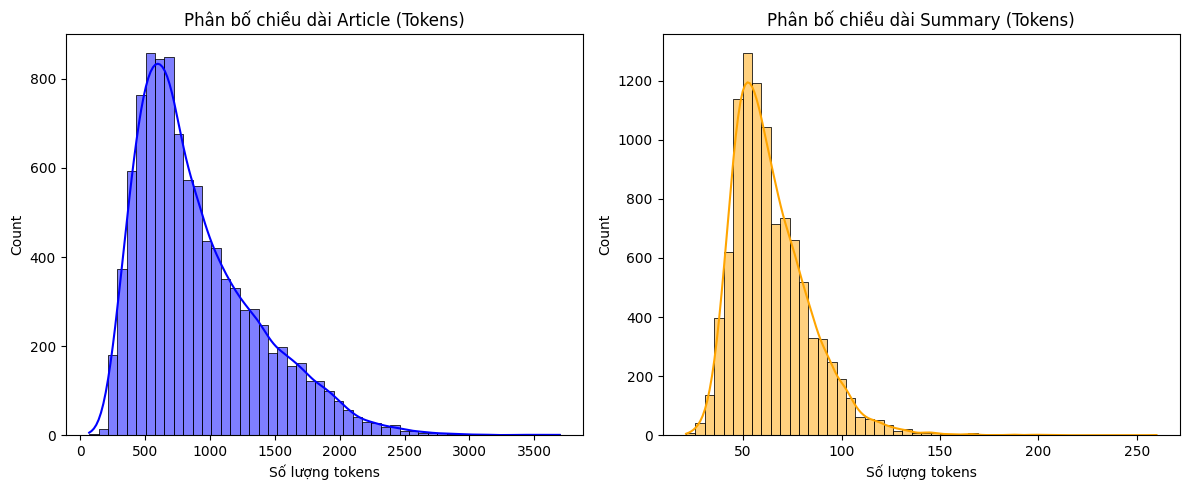
\includegraphics[width=0.80\textwidth]{Images/tokens_figure.png}
    \caption{Phân phối số lượng token (syllable-level) của Article (trái) và Summary (phải) trong tập VietNews.}
    \label{fig:token_dist}
\end{figure}

Như Hình \ref{fig:token_dist} cho thấy, phân phối độ dài Article có dạng lệch phải (right-skewed) với đỉnh chính ở khoảng 500--700 tokens. Phần lớn bài báo nằm trong khoảng 400--800 tokens, tuy nhiên phần đuôi dài (long tail) kéo dài đến trên 3,500 tokens, cho thấy sự tồn tại đáng kể của các bài viết dài vượt xa ngưỡng truncation 512 tokens mà BARTpho sử dụng trong huấn luyện. Ở phía biểu đồ Summary, phân phối tập trung hẹp hơn đáng kể với đỉnh khoảng 50--70 tokens và phần lớn mẫu nằm trong khoảng 40--100 tokens. Dựa trên đỉnh phân phối (Article $\sim$500--700 tokens, Summary $\sim$50--70 tokens), tỷ lệ nén (compression ratio) ước tính vào khoảng 7:1 đến 14:1, đòi hỏi mô hình phải có khả năng chắt lọc thông tin trọng tâm thay vì chỉ cắt bớt nội dung.

Đáng lưu ý, do sử dụng syllable-level tokenizer, cùng một đoạn văn bản tiếng Việt sẽ tạo ra nhiều token hơn khoảng 1.3--1.5 lần so với word-level tokenizer\footnote{Ước tính thực nghiệm: tiếng Việt trung bình 1.3--1.5 âm tiết/từ do cấu trúc đơn âm tiết chiếm ưu thế, nhưng nhiều từ ghép gồm 2 âm tiết (ví dụ: ``công nghệ'', ``nghiên cứu'').}. Điều này có nghĩa rằng ngưỡng 512 syllable tokens mà BARTpho sử dụng chỉ bao phủ khoảng 340--390 từ thực tế, trong khi phân phối cho thấy phần lớn bài báo vượt con số này. Sự tồn tại của đuôi dài trong phân phối Article chính là động lực cốt lõi cho thử nghiệm so sánh Map-Reduce và Native Long-Context trong nghiên cứu này.

\subsection{Chiến lược Lấy mẫu và Tiền xử lý}
Nhằm tối ưu tài nguyên phần cứng (Kaggle GPU T4 16GB, VRAM giới hạn) đồng thời đảm bảo chất lượng dữ liệu huấn luyện, chúng tôi áp dụng quy trình lấy mẫu và lọc dữ liệu nhiều bước. Từ toàn bộ tập VietNews (150,736 mẫu), dữ liệu được xáo trộn ngẫu nhiên với seed cố định ($\text{seed} = 42$), sau đó chọn 30,000 mẫu đầu tiên làm tập ứng viên. Trên tập này, chúng tôi áp dụng bộ lọc Lead-Bias theo phương pháp Data-centric AI: các mẫu mà bản tóm tắt chuẩn có tỷ lệ trùng lặp từ vựng (word overlap) với ba câu đầu tiên của bài báo $\geq 80\%$ được loại bỏ, nhằm giảm thiên lệch Lead Bias trong dữ liệu huấn luyện -- nếu giữ lại những mẫu này, mô hình sẽ học cách sao chép đoạn mở đầu thay vì thực sự tóm tắt. Sau bước lọc, số lượng mẫu đạt tiêu chuẩn vượt 12,000, từ đó chúng tôi lấy chính xác 12,000 mẫu và chia thành: 10,000 mẫu huấn luyện, 1,000 mẫu xác thực, và 1,000 mẫu kiểm thử (General Set). Quy trình tiền xử lý bổ sung bao gồm: (1) Chuẩn hóa Unicode tiếng Việt, (2) Loại bỏ thẻ HTML nhiễu, (3) Loại bỏ khoảng trắng thừa, và (4) Lọc bỏ các mẫu có văn bản rỗng. Từ tập kiểm thử, chúng tôi lọc ra một tập con gồm các bài báo có độ dài $\geq 800$ từ (Long Document Set, $n = 69$) để đánh giá riêng năng lực xử lý ngữ cảnh dài. Toàn bộ các mô hình đều được huấn luyện và đánh giá trên cùng một tập dữ liệu cố định nhằm đảm bảo tính công bằng trong so sánh.

\subsection{Cấu hình Huấn luyện}
Bảng \ref{tab:training_config} tổng hợp toàn bộ siêu tham số huấn luyện cho ba cấu hình thực nghiệm. Tất cả các thí nghiệm đều sử dụng độ chính xác hỗn hợp FP16 và weight decay 0.01. Đáng chú ý, tốc độ học (learning rate) của LoRA ($3 \times 10^{-4}$ cho BARTpho, $2 \times 10^{-4}$ cho Qwen2.5) được đặt cao hơn 10--15 lần so với Full Fine-Tuning ($2 \times 10^{-5}$). Sự khác biệt này tuân theo khuyến nghị của Hu et al. \cite{lora}: do LoRA chỉ cập nhật các ma trận hạng thấp $A$ và $B$ (chiếm dưới 5\% tổng tham số), mỗi bước cập nhật cần biên độ lớn hơn để đạt tốc độ hội tụ tương đương. Ngoài ra, Qwen2.5 sử dụng optimizer AdamW-8bit \cite{qlora} để giảm bộ nhớ optimizer trên GPU 16GB, và gradient checkpointing để đánh đổi tốc độ tính toán lấy bộ nhớ.

\begin{table}[H]
\centering
\caption{Tổng hợp siêu tham số huấn luyện cho ba cấu hình thực nghiệm.}
\label{tab:training_config}
\begin{tabular}{@{}lccc@{}}
\toprule
\textbf{Tham số} & \textbf{FFT BARTpho} & \textbf{LoRA BARTpho} & \textbf{LoRA Qwen2.5} \\
\midrule
Model checkpoint       & \multicolumn{2}{c}{\texttt{vinai/bartpho-syllable}} & \texttt{Qwen/Qwen2.5-0.5B} \\
Learning rate          & $2 \times 10^{-5}$ & $3 \times 10^{-4}$ & $2 \times 10^{-4}$ \\
LR scheduler           & Cosine & Cosine & Linear \\
Warmup                  & 10\% steps & Default & Default \\
Optimizer               & AdamW & AdamW & AdamW-8bit \\
Epochs                  & 4 & 5 & 4 \\
Batch size (per device) & 4 & 8 & 1 \\
Gradient accumulation   & 4 & 2 & 8 \\
Effective batch size    & 16 & 16 & 8 \\
Max input length        & 512 & 512 & 2048 \\
Max target length       & 128 & 128 & 128 \\
Precision               & FP16 & FP16 & FP16 \\
Gradient checkpointing  & -- & -- & Có \\
\bottomrule
\end{tabular}
\end{table}

Cần lưu ý rằng BARTpho được tiền huấn luyện với $\text{max\_position\_embeddings} = 1024$, nghĩa là các Learned Absolute Position Embeddings cho vị trí 0--1023 đã được học sẵn trong quá trình tiền huấn luyện trên 20GB dữ liệu tiếng Việt. Trong quá trình tinh chỉnh, chúng tôi giới hạn $\text{max\_input\_length} = 512$ do ràng buộc bộ nhớ GPU T4 (16GB) -- đây là chiến lược phổ biến nhằm tăng batch size hiệu dụng và tốc độ hội tụ. Khi suy luận, ngưỡng truncation được nới lên 1024 tokens để tận dụng toàn bộ dải vị trí đã được tiền huấn luyện. Mặc dù các vị trí 512--1023 (0-indexed) không được cập nhật trong quá trình tinh chỉnh cho nhiệm vụ tóm tắt, kiến thức vị trí từ giai đoạn tiền huấn luyện vẫn được bảo toàn, cho phép mô hình xử lý chuỗi dài hơn so với ngưỡng huấn luyện mà không gây lỗi ngoại suy.

\subsection{Cấu hình Suy luận và Giải mã}

Bảng \ref{tab:decoding_config} trình bày cấu hình giải mã cho pha đánh giá. Trong nghiên cứu này, chúng tôi sử dụng Beam Search với $\text{num\_beams} = 4$ làm chiến lược giải mã chuẩn cho tất cả các mô hình, theo khuyến nghị phổ biến trong các bài toán sinh văn bản có điều kiện \cite{bart_original}. Beam Search cân bằng giữa chất lượng đầu ra (tìm kiếm chuỗi có xác suất cao nhất) và chi phí tính toán, trong khi các phương pháp sampling (Top-$k$, Top-$p$) thường gây biến thiên lớn hơn do tính ngẫu nhiên nội tại. Trên tập Long Document Set, $\text{length\_penalty} = 2.0$ được áp dụng cho BARTpho nhằm khuyến khích sinh văn bản dài hơn, phù hợp với độ dài nhãn chuẩn của các bài viết dài.

\begin{table}[H]
\centering
\caption{Cấu hình giải mã (Decoding) cho các pha đánh giá.}
\label{tab:decoding_config}
\begin{tabular}{@{}lccc@{}}
\toprule
\textbf{Tham số} & \textbf{BARTpho (General)} & \textbf{BARTpho (Long)} & \textbf{Qwen2.5} \\
\midrule
Decoding method     & Beam Search & Beam Search & Beam Search \\
num\_beams          & 4 & 4 & 4 \\
max\_length         & 128 & 150 & -- \\
max\_new\_tokens    & -- & -- & 128 / 150 \\
length\_penalty     & 1.0 & 2.0 & 1.0 \\
Input truncation    & 1024 & 1024 / SW 512 & 2048 \\
\bottomrule
\end{tabular}
\end{table}

\subsection{Các Độ đo Đánh giá}

\textbf{ROUGE} (Recall-Oriented Understudy for Gisting Evaluation) \cite{rouge_original} đo lường mức độ trùng khớp n-gram giữa kết quả sinh ra và nhãn chuẩn, thiên về Recall:
\begin{equation}
    \text{ROUGE-N} = \frac{\sum_{S_{ref}} \sum_{gram_n \in S_{ref}} Count_{match}(gram_n)}{\sum_{S_{ref}} \sum_{gram_n \in S_{ref}} Count(gram_n)}
\end{equation}
Chúng tôi báo cáo ROUGE-1 (unigram, phản ánh khả năng bao phủ từ vựng), ROUGE-2 (bigram, phản ánh mức độ khớp cụm từ liên tiếp), và ROUGE-L (dựa trên chuỗi con chung dài nhất -- Longest Common Subsequence, phản ánh cấu trúc câu).

\textbf{BLEU-4} (Bilingual Evaluation Understudy) \cite{bleu_original} tập trung vào Precision của n-gram, kèm hình phạt độ dài (Brevity Penalty) để phạt các bản tóm tắt quá ngắn:
\begin{equation}
    \text{BLEU} = BP \cdot \exp\left( \sum_{n=1}^N w_n \log p_n \right), \quad BP = \begin{cases} 1 & \text{nếu } c > r \\ e^{(1 - r/c)} & \text{nếu } c \leq r \end{cases}
\end{equation}
trong đó $c$ là chiều dài văn bản sinh ra, $r$ là chiều dài văn bản chuẩn, $p_n$ là precision cho n-gram bậc $n$, và $w_n = 1/N$ là trọng số đều cho mỗi bậc n-gram. Nghiên cứu sử dụng $N=4$ (BLEU-4), cấu hình chuẩn trong các bài toán sinh văn bản. Khác với ROUGE (thiên Recall), BLEU phản ánh mức độ trôi chảy ngữ pháp và tính chính xác của các cụm từ liên tiếp mà mô hình sinh ra.

\textbf{BERTScore} \cite{bertscore} đo lường tương đồng ngữ nghĩa bằng cách tính Cosine similarity cực đại giữa các token embeddings từ mô hình BERT tiền huấn luyện (trong nghiên cứu này là \texttt{bert-base-multilingual-cased}):
\begin{equation}
    R_{BERT} = \frac{1}{|x|} \sum_{x_i \in x} \max_{\hat{x}_j \in \hat{x}} \frac{x_i^\top \hat{x}_j}{\|x_i\| \cdot \|\hat{x}_j\|}
\end{equation}
Chỉ số này bổ khuyết cho ROUGE và BLEU bằng cách cho phép đánh giá trường hợp mô hình sử dụng từ đồng nghĩa hoặc paraphrase mà không bị phạt bởi các thang đo đếm từ chính xác. Tuy nhiên, do sử dụng mô hình đa ngôn ngữ thay vì mô hình chuyên biệt cho tiếng Việt, độ chính xác của BERTScore có thể bị ảnh hưởng ở mức độ nhất định.

%======================================================================
\section{Kết quả và Bàn luận}
\label{sec:results}
%======================================================================

\subsection{Đánh giá So sánh Tổng thể trên Tập Kiểm thử Chung}\label{sec:general_eval}

Bảng \ref{tab:general_eval} trình bày kết quả đánh giá trên toàn bộ 1,000 bài báo của tập kiểm thử chung (General Set). Ở đây, chúng tôi tổng hợp đồng thời cả ba nhánh phương pháp: các baseline trích xuất truyền thống, kiến trúc Transformer tùy chỉnh (huấn luyện từ đầu) và các mô hình tiền huấn luyện SOTA.

\begin{table*}[htbp]
\centering
\caption{Kết quả đánh giá trên tập kiểm thử chung (General Set, $n = 1{,}000$). Giá trị in đậm biểu thị kết quả tốt nhất trên từng cột.}
\label{tab:general_eval}
  \resizebox{\textwidth}{!}{
  \begin{tabular}{@{}lccccc@{}}
\toprule
\textbf{Phương pháp} & \textbf{ROUGE-1} & \textbf{ROUGE-2} & \textbf{ROUGE-L} & \textbf{BLEU} & \textbf{BERTScore-F1} \\
\midrule
Lead-3                     & 45.75 & 21.87 & 28.99 & 8.79 & \textbf{72.69} \\
TextRank                   & 36.88 & 18.99 & 24.94 & 6.37 & 71.52 \\
\midrule
\textit{Các biến thể Transformer tùy chỉnh (Huấn luyện từ đầu):} & & & & & \\
Baseline Transformer (6L) & 34.37 & 8.05 & 22.13 & 0.52 & 65.08 \\
Improved Core (RoPE + RMSNorm) & 46.00 & 10.46 & 27.59 & 1.82 & 68.99 \\
Extended (11L + Weight Tying) & 47.30 & 12.84 & 28.97 & 2.26 & 70.15 \\
Entity Guided & 48.79 & 13.19 & 29.50 & 2.54 & 70.34 \\
Entity Guided + GTF-Penalty & 50.00 & 14.01 & 29.74 & 2.57 & 70.88 \\
\midrule
FFT -- BARTpho             & 50.24 & 15.27 & 30.52 & 2.25 & 66.46 \\
LoRA -- BARTpho            & 50.17 & 14.93 & 30.40 & 2.34 & 66.29 \\
LoRA -- Qwen2.5            & 47.85 & 20.42 & 30.22 & 9.19 & 70.34 \\
LoRA -- Qwen2.5 + GTF      & \textbf{51.28} & \textbf{23.05} & \textbf{31.26} & \textbf{10.29} & 72.52 \\
\bottomrule
\end{tabular}}
\end{table*}

\begin{figure}[H]
    \centering
    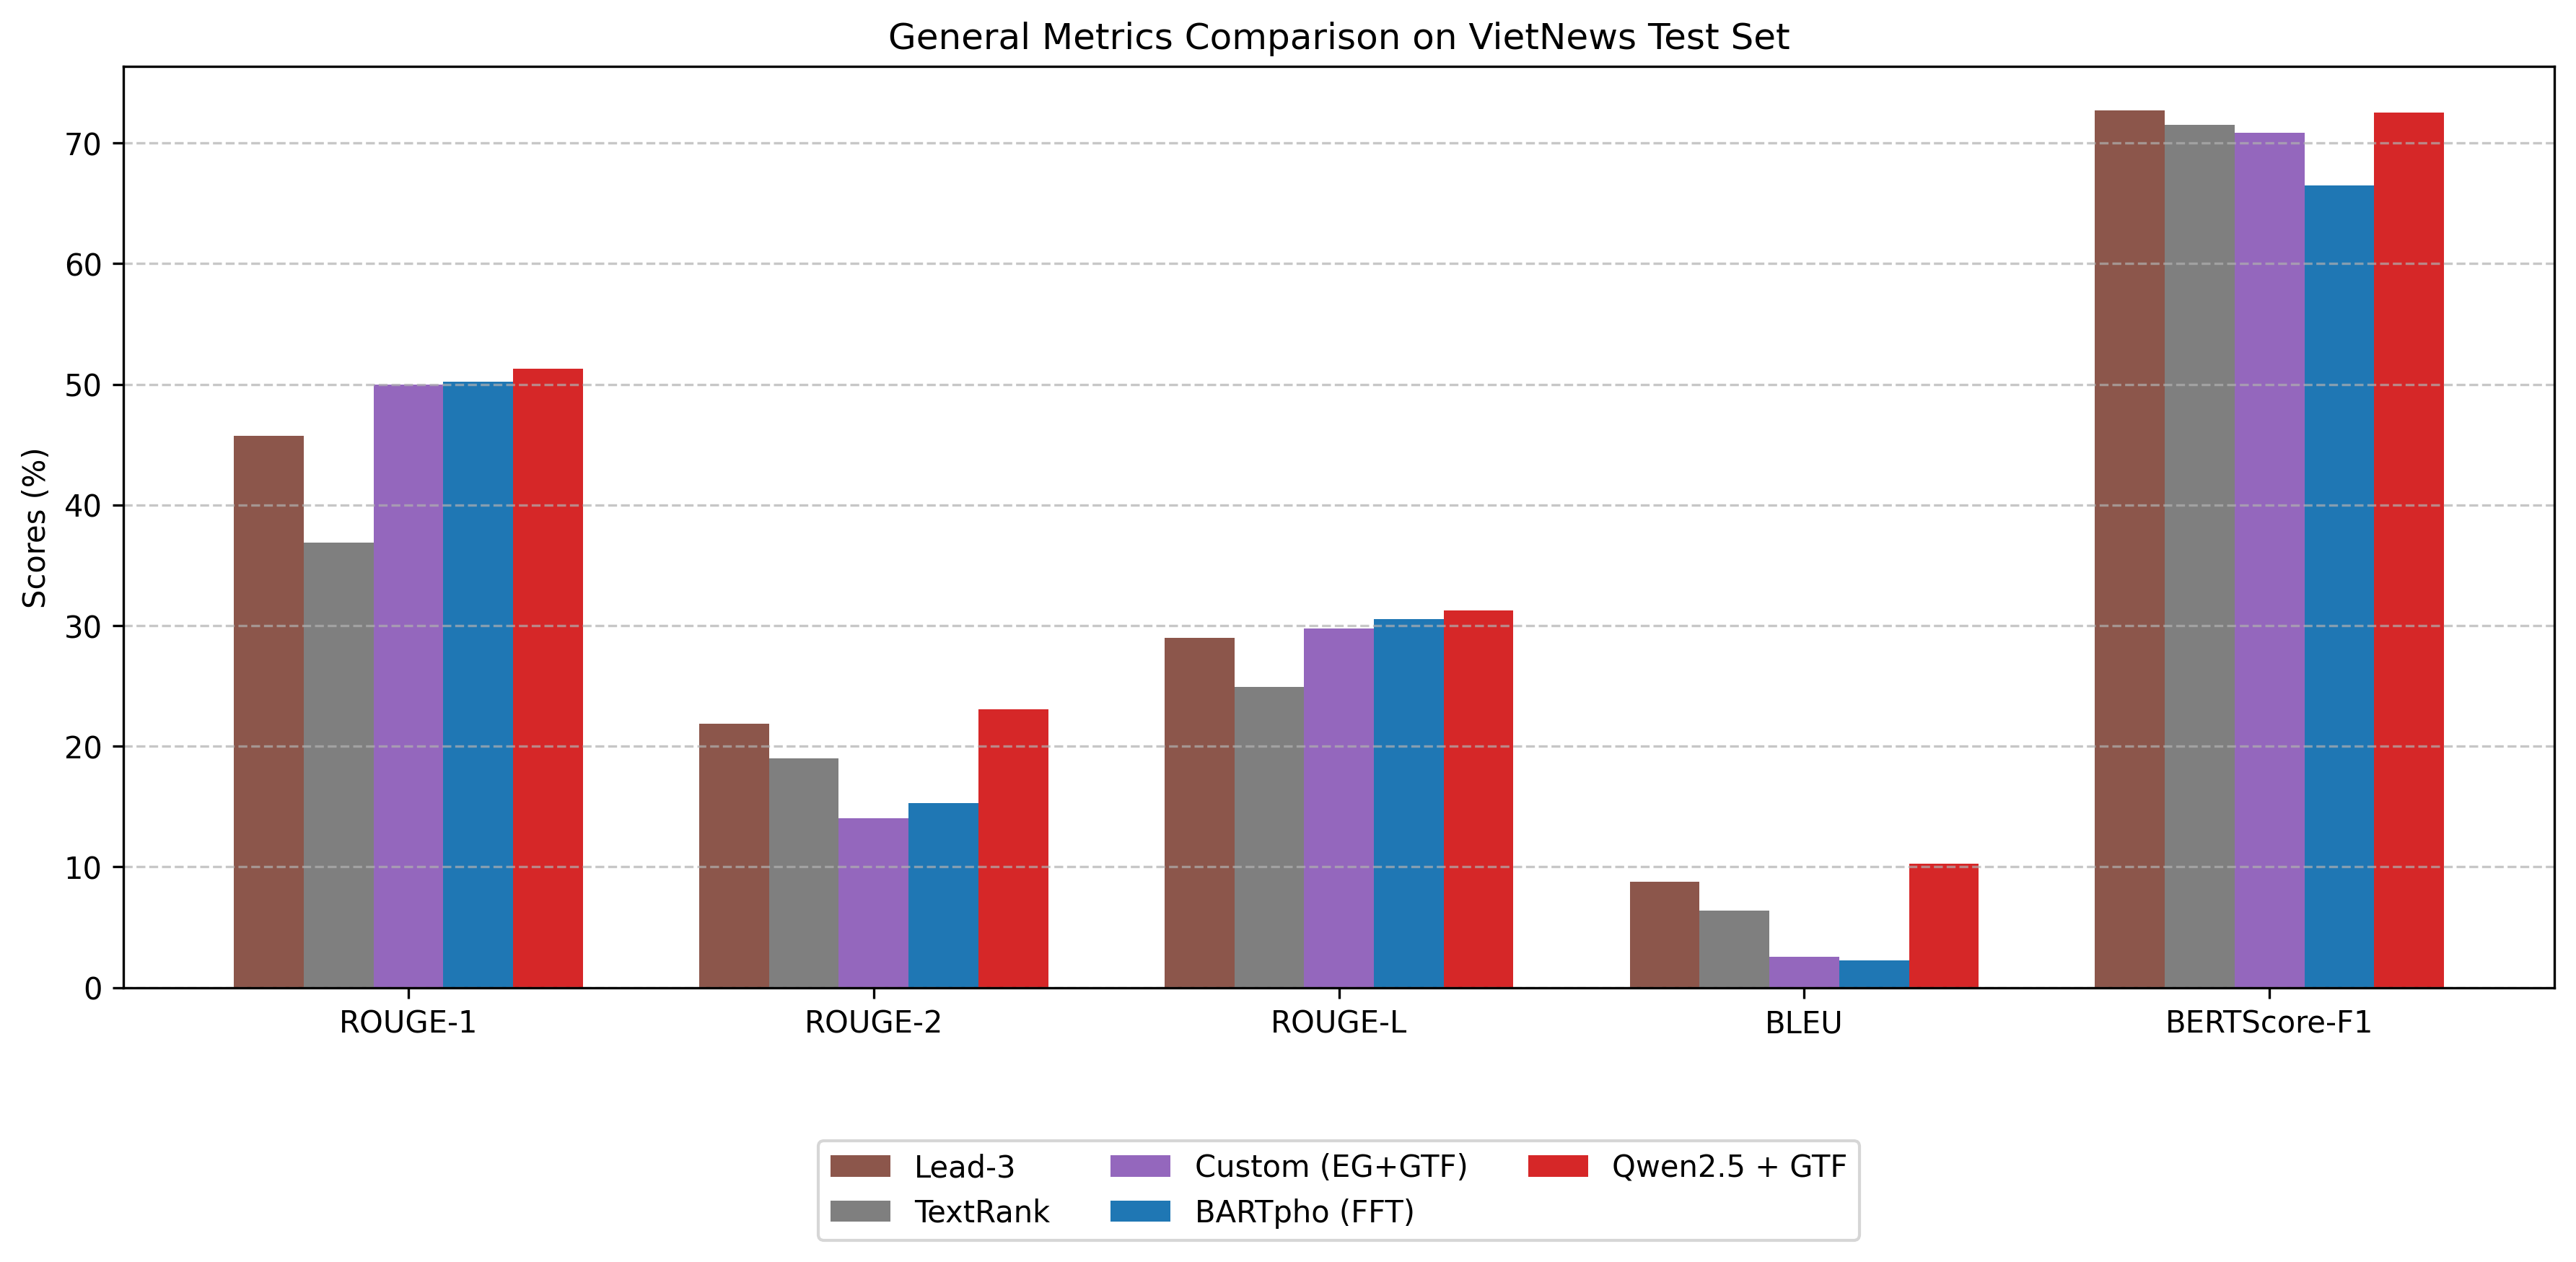
\includegraphics[width=\textwidth]{Images/general_metrics.png}
    \caption{Trực quan hóa hiệu năng các mô hình trên tập kiểm thử chung (biểu đồ cột).}
    \label{fig:general}
\end{figure}

Hình \ref{fig:radar} trình bày biểu đồ radar cho phép quan sát `hồ sơ hiệu năng'''' (performance profile) tổng thể của các phương pháp. Đáng chú ý, Custom Transformer thể hiện một cấu hình đa giác cực kỳ dị biệt: đỉnh đồ thị vươn rất dài ở trục ROUGE-1 (50.00, tiệm cận các SOTA) nhưng lại co cụm gần như về 0 ở các trục BLEU và ROUGE-2. Sự bất cân xứng dị thường này chính là biểu hiện trực quan của \textit{Nghịch lý ROUGE} (sẽ được phân tích sâu qua lăng kính LLM Judge ở mục \ref{sec:llm_judge}): mô hình chỉ học được cách trích xuất từ khóa rời rạc mà hoàn toàn thiếu vắng khả năng liên kết cú pháp (thể hiện qua BLEU cực thấp). Trong khi đó, Qwen2.5+GTF thể hiện một đa giác bao trùm và cân đối nhất trên tất cả các trục.

\begin{figure}[H]
    \centering
    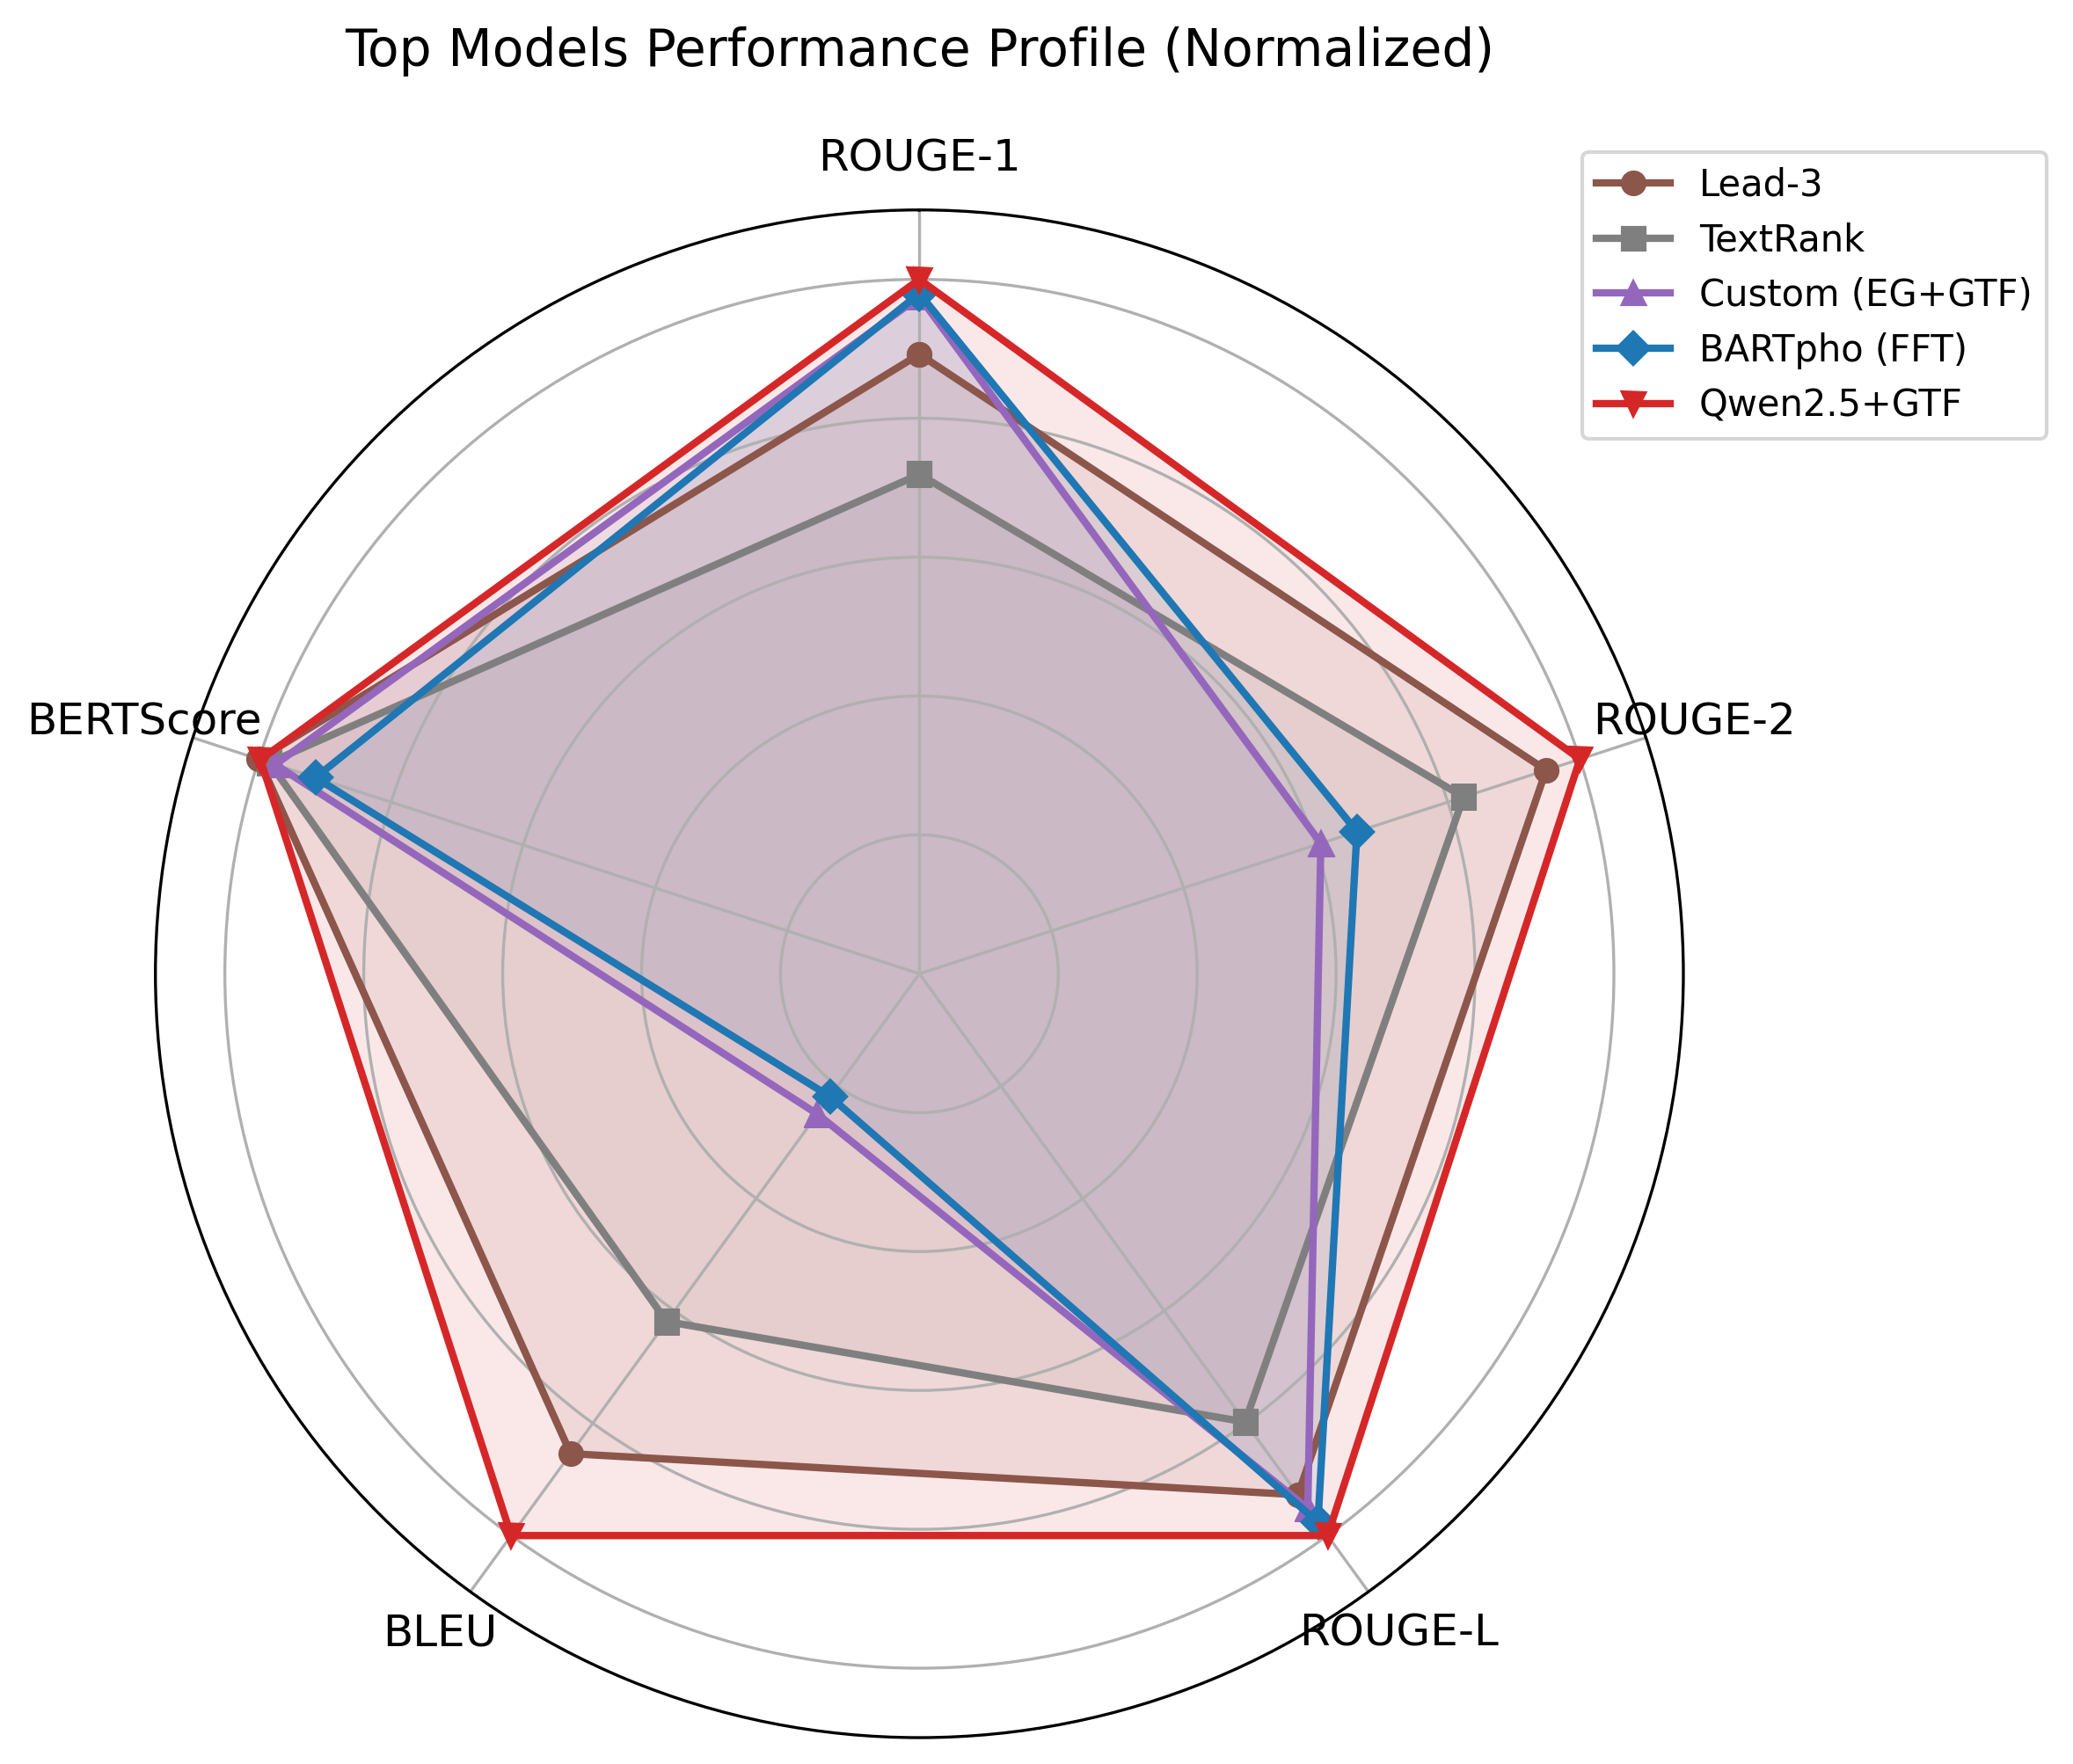
\includegraphics[width=0.9\textwidth]{Images/radar_chart_models.png}
    \caption{Biểu đồ radar so sánh hồ sơ hiệu năng (đã chuẩn hóa). Custom Transformer bị biến dạng mạnh (cao ở ROUGE-1, cực thấp ở BLEU), minh họa trực quan cho nghịch lý N-gram. Qwen2.5+GTF là mô hình toàn diện nhất.}
    \label{fig:radar}
\end{figure}

\paragraph{Hiện tượng Lead Bias.}
Kết quả đáng chú ý nhất trong Bảng \ref{tab:general_eval} là phương pháp Lead-3 đạt ROUGE-2 (21.87), BLEU (8.79) và BERTScore-F1 (72.69) cao hơn đáng kể so với các mô hình học sâu. Hiện tượng này phản ánh đặc tính Lead Bias \cite{lead_bias} của văn bản báo chí: phần lớn tóm tắt chuẩn do con người viết thực chất được sao chép hoặc biến tấu nhẹ từ phần mở bài (Sapo). Vì Lead-3 trích xuất nguyên văn các câu đầu, các chuỗi n-gram liên tiếp được giữ nguyên, giải thích cho điểm BLEU và ROUGE-2 cao. Phát hiện này nhất quán với kết luận của Kryściński et al. \cite{lead_bias} rằng Lead Bias là hiện tượng phổ biến trong các bộ dữ liệu tin tức và cần được cân nhắc kỹ khi diễn giải kết quả.

\paragraph{Giới hạn của cải tiến kiến trúc và "Nghịch lý ROUGE".}
Bảng \ref{tab:general_eval} cho thấy sự thay đổi hiệu năng của Custom Transformer qua các bản cập nhật kiến trúc. Việc áp dụng RoPE, RMSNorm, SwiGLU và tăng số lớp (11 lớp, Weight Tying) cải thiện ROUGE-1 từ 34.37 lên 47.30. Khi tích hợp Entity Guided và GTF-Penalty, ROUGE-1 đạt mức 50.00, tiệm cận hiệu năng của các mô hình ngôn ngữ lớn (LLMs).

Tuy nhiên, khoảng cách lớn giữa ROUGE-1 (50.00) và các chỉ số đo lường độ trôi chảy như BLEU (2.57) hay LLM-as-a-Judge (1.05, Mục \ref{sec:llm_judge}) cho thấy điểm yếu của việc dùng ROUGE làm thước đo duy nhất. Do tập dữ liệu huấn luyện nhỏ, Custom Transformer chưa đủ khả năng mô hình hóa cú pháp (syntactic parsing) và ngữ nghĩa (semantic coherence) như BARTpho hay Qwen2.5. Thay vào đó, Entity Guided và GTF-Penalty giúp mô hình tối ưu độ trùng lặp N-gram bằng cách trích xuất từ khóa, nhưng không thể sắp xếp chúng thành câu hoàn chỉnh, tạo ra các chuỗi từ vựng rời rạc (word salad). Kết quả này cho thấy: (1) các mô hình có thể dễ dàng đạt điểm cao trên những độ đo heuristic (như ROUGE) thông qua tinh chỉnh kiến trúc mà không thực sự hiểu ngôn ngữ; (2) để sinh văn bản trôi chảy và logic, tri thức tiền huấn luyện (pre-training) trên tập dữ liệu lớn vẫn là yếu tố bắt buộc.

\paragraph{BARTpho: bao phủ từ vựng tốt nhưng hạn chế về độ trôi chảy.}
BARTpho đạt mức ROUGE-1 khá cao (FFT: 50.24, với Khoảng tin cậy 95\% CI: [49.72, 50.76]), cho thấy mô hình có khả năng bao phủ từ vựng rộng nhờ cơ chế Bidirectional Attention của Encoder. Tuy nhiên, BLEU của BARTpho chỉ đạt 2.25, thấp hơn đáng kể so với Lead-3 (8.79) -- khoảng cách lên đến 6.54 điểm. Hiện tượng này phản ánh hạn chế của mô hình Seq2Seq khi sinh văn bản trừu tượng: quá trình diễn giải lại (paraphrase) tạo ra các chuỗi n-gram khác biệt so với nhãn chuẩn, dẫn đến Precision thấp. BERTScore của BARTpho (66.46) cũng thấp hơn cả TextRank (71.52) và Lead-3 (72.69), cho thấy chất lượng ngữ nghĩa tổng thể chưa đạt mức của phương pháp trích xuất.

\paragraph{Qwen2.5 và sức mạnh của GTF-Penalty.}
Qwen2.5 nguyên bản (chỉ tinh chỉnh LoRA) gặp phải hiện tượng lặp từ phổ biến ở cấu trúc Causal Decoder, khiến ROUGE-1 chỉ đạt 47.85. Tuy nhiên, khi kết hợp giải mã với thuật toán \textit{Generative Token Frequency (GTF) Penalty}, hiệu năng sinh văn bản bùng nổ mạnh mẽ. Phiên bản \textbf{Qwen2.5 + GTF} thiết lập mức trần (SOTA) mới trên mọi chỉ số sinh: ROUGE-1 đạt 51.28 (vượt qua hoàn toàn cả BARTpho), ROUGE-2 đạt 23.05 và BLEU đạt 10.29 (vượt xa mức trích xuất tĩnh của Lead-3). Việc can thiệp trực tiếp vào Logits bằng cách phạt các token sinh lặp (nhưng không phạt các token thuộc về văn bản gốc) đã giải phóng hoàn toàn sức mạnh tiền huấn luyện 18 nghìn tỷ token của Qwen2.5. Các chỉ số này phản ánh khả năng vừa sinh văn bản trừu tượng, mượt mà mà vẫn giữ được độ liên kết cấu trúc n-gram ở mức độ rất cao. Điểm BERTScore của Qwen2.5+GTF (72.52) cũng tiệm cận mức của Lead-3 (72.69).

\paragraph{Tính tương thích của GTF-Penalty với Causal LM.}
Thuật toán GTF-Penalty được thiết kế đặc thù cho Qwen2.5 và Custom Transformer thay vì BARTpho do sự khác biệt trong cơ chế Attention. Ở mô hình Seq2Seq như BARTpho, luồng Cross-Attention hoạt động độc lập, cho phép Decoder tham chiếu liên tục với biểu diễn ngữ cảnh tĩnh từ Encoder, giúp hạn chế tình trạng lặp từ. Ngược lại, kiến trúc Decoder-only của Qwen2.5 xử lý cả văn bản đầu vào và tóm tắt đầu ra trong cùng một không gian Self-Attention. Quá trình sinh tự hồi quy (auto-regressive) của cấu trúc này nhạy cảm hơn với hiện tượng \textit{Exposure Bias}; khi một từ lặp xuất hiện, mô hình có xu hướng tăng cường trọng số chú ý vào chính chuỗi lặp đó. 

Về mặt kỹ thuật, GTF-Penalty yêu cầu quyền truy cập vào chuỗi token tổng hợp \texttt{[Prompt + Generated]} để tính toán hình phạt đối với phần văn bản sinh ra, đồng thời bảo toàn các thực thể (entities) được sao chép từ bài báo gốc. Luồng thông tin tích hợp này có sẵn trong Causal LM nhưng bị cô lập ở khâu xử lý của Decoder trong mô hình Seq2Seq. Việc áp dụng GTF-Penalty giúp kiểm soát đặc tính lặp từ của Causal LM, từ đó cải thiện chất lượng sinh văn bản mà không làm thay đổi trọng số cốt lõi của mô hình tiền huấn luyện.

\paragraph{LoRA so với Full Fine-Tuning.}
Kết quả cho thấy LoRA trên BARTpho (ROUGE-1: 50.17) đạt hiệu năng tiệm cận FFT (ROUGE-1: 50.24), với chênh lệch chỉ 0.07 điểm ($\Delta = 0.14\%$). Trên BLEU, LoRA thậm chí cao hơn nhẹ (2.34 so với 2.25). Xét đến việc LoRA giảm trên 95\% số lượng tham số cần cập nhật, kết quả này cho thấy kỹ thuật PEFT rất hiệu quả trong các bài toán tóm tắt tiếng Việt. Điều này đồng thuận với kết luận của Hu et al. \cite{lora} rằng không gian cập nhật hiệu quả thường có chiều thấp hơn nhiều so với toàn bộ không gian tham số.

\subsection{Phân tích Ảnh hưởng của Chiến lược Giải mã}

Trong quá trình sinh văn bản tự động, chiến lược giải mã (decoding strategy) là yếu tố quan trọng trong việc kiểm soát tính đa dạng và độ chính xác của từ vựng được chọn. Bảng \ref{tab:decoding_eval} trình bày kết quả thử nghiệm các chiến lược giải mã khác nhau trên mô hình BARTpho (Full Fine-Tuning) bao gồm phương pháp tất định (Greedy, Beam Search) và phương pháp lấy mẫu (Top-k, Top-p).

\begin{table}[H]
\centering
\caption{Ảnh hưởng của các chiến lược giải mã khác nhau đến chất lượng và thời gian sinh tóm tắt trên mô hình BARTpho.}
\label{tab:decoding_eval}
\resizebox{\columnwidth}{!}{
\begin{tabular}{@{}lccccccc@{}}
\toprule
\textbf{Chiến lược} & \textbf{ROUGE-1} & \textbf{ROUGE-2} & \textbf{ROUGE-L} & \textbf{BLEU} & \textbf{BERT-F1} & \textbf{Thời gian (phút)} \\
\midrule
Greedy & 49.69 & \textbf{15.42} & \textbf{30.73} & 2.21 & \textbf{66.91} & \textbf{15.7} \\
Beam Search ($k=4$) & 50.24 & 15.26 & 30.53 & \textbf{2.25} & 66.46 & 24.5 \\
Beam Search ($k=8$) & 50.20 & 14.91 & 30.34 & 2.21 & 66.20 & 41.0 \\
Top-k ($k=50$) & \textbf{50.34} & 13.69 & 29.54 & 1.65 & 66.22 & 16.6 \\
Top-p ($p=0.9$) & 49.72 & 13.81 & 29.28 & 1.78 & 66.36 & 16.2 \\
Top-p ($p=0.95$) & 50.04 & 13.39 & 29.17 & 1.76 & 66.11 & 16.8 \\
\bottomrule
\end{tabular}
}
\end{table}

Kết quả thực nghiệm cho thấy một sự đánh đổi rõ rệt giữa chất lượng, tốc độ và tính đa dạng từ vựng trong nhiệm vụ tóm tắt. Cụ thể:

Thứ nhất, đối với nhiệm vụ tóm tắt vốn đòi hỏi tính ràng buộc cao và sự trung thành với văn bản gốc, các chiến lược tất định (Deterministic) như Greedy Search và Beam Search thể hiện sự ưu việt hơn so với các chiến lược lấy mẫu (Stochastic) như Top-k và Top-p. Mặc dù Top-k ($k=50$) đạt đỉnh ROUGE-1 (50.34), sự suy giảm mạnh ở các chỉ số đánh giá cấu trúc n-gram (ROUGE-2 chỉ đạt 13.69, BLEU giảm xuống 1.65) cho thấy việc lấy mẫu ngẫu nhiên đôi khi phá vỡ tính mạch lạc của câu văn tiếng Việt.

Thứ hai, hiện tượng ``Beam Search Curse'' (sự suy giảm chất lượng khi kích thước chùm tia quá lớn) được quan sát rõ ràng. Việc tăng kích thước Beam từ 4 lên 8 không những làm tăng thời gian suy luận lên 1.67 lần (từ 24.5 phút lên 41.0 phút), mà còn làm giảm toàn bộ các hệ số chất lượng (ROUGE-1 giảm từ 50.24 xuống 50.20, BLEU giảm từ 2.25 xuống 2.21). Điều này xảy ra do chùm tia lớn có xu hướng ưu tiên các chuỗi mang tính khái quát, ngắn gọn hoặc an toàn quá mức, làm mất đi các chi tiết quan trọng trong bản tóm tắt.

Thứ ba, Greedy Search chứng minh hiệu năng cao trong bài toán này. Là phương pháp nhanh nhất (15.7 phút), Greedy Search lại đạt kết quả tốt nhất ở ROUGE-2 (15.42), ROUGE-L (30.73), và BERTScore-F1 (66.91). Điều này gợi ý rằng không gian xác suất đầu ra của BARTpho sau khi tinh chỉnh đã phân bố rất tập trung (sharp distribution), khiến việc tìm kiếm mở rộng (như Beam Search) mang lại ít lợi ích so với chi phí tính toán bỏ ra. Dựa trên phân tích này, chúng tôi chọn Beam Search ($k=4$) làm cấu hình cân bằng chuẩn cho các so sánh tổng thể, và Greedy Search như một sự thay thế tối ưu trong các hệ thống yêu cầu độ trễ thấp.



\subsection{Đánh giá trên Tập Văn bản Dài}

Bảng \ref{tab:long_eval} và Hình \ref{fig:long} trình bày kết quả trên tập Long Document Set (các bài báo $\geq 800$ từ), nhằm trả lời trực tiếp câu hỏi nghiên cứu RQ3. Phần đánh giá này tập trung so sánh các chiến lược xử lý ngữ cảnh dài giữa BARTpho và Qwen2.5, do đó các phương pháp trích xuất (Lead-3, TextRank) không được đưa vào bảng so sánh vì bản chất của chúng không bị ảnh hưởng bởi giới hạn ngữ cảnh -- phương pháp trích xuất chọn câu nguyên văn và không phụ thuộc vào cửa sổ ngữ cảnh của mô hình.

\begin{table*}[htbp]
\centering
  \caption{Kết quả đánh giá trên tập văn bản dài (Long Document Set, bài báo $\geq 800$ từ, $n = 69$). Giá trị in đậm biểu thị kết quả tốt nhất trên từng cột.}
  \label{tab:long_eval}
  \resizebox{\textwidth}{!}{
  \begin{tabular}{@{}lccccc@{}}
\toprule
\textbf{Phương pháp} & \textbf{ROUGE-1} & \textbf{ROUGE-2} & \textbf{ROUGE-L} & \textbf{BLEU} & \textbf{BERTScore-F1} \\
\midrule
FFT -- BARTpho (Truncation 1024)    & \textbf{47.79} & 12.05 & 26.94 & 1.22 & 63.64 \\
FFT -- BARTpho (Map-Reduce Sliding Window) & 47.05 & 12.49 & 26.16 & 0.64 & 62.98 \\
LoRA -- Qwen2.5 (Native 2048)       & 45.38 & \textbf{16.81} & \textbf{27.06} & \textbf{6.27} & \textbf{68.94} \\
\bottomrule
\end{tabular}}
\end{table*}

\begin{figure}[H]
    \centering
    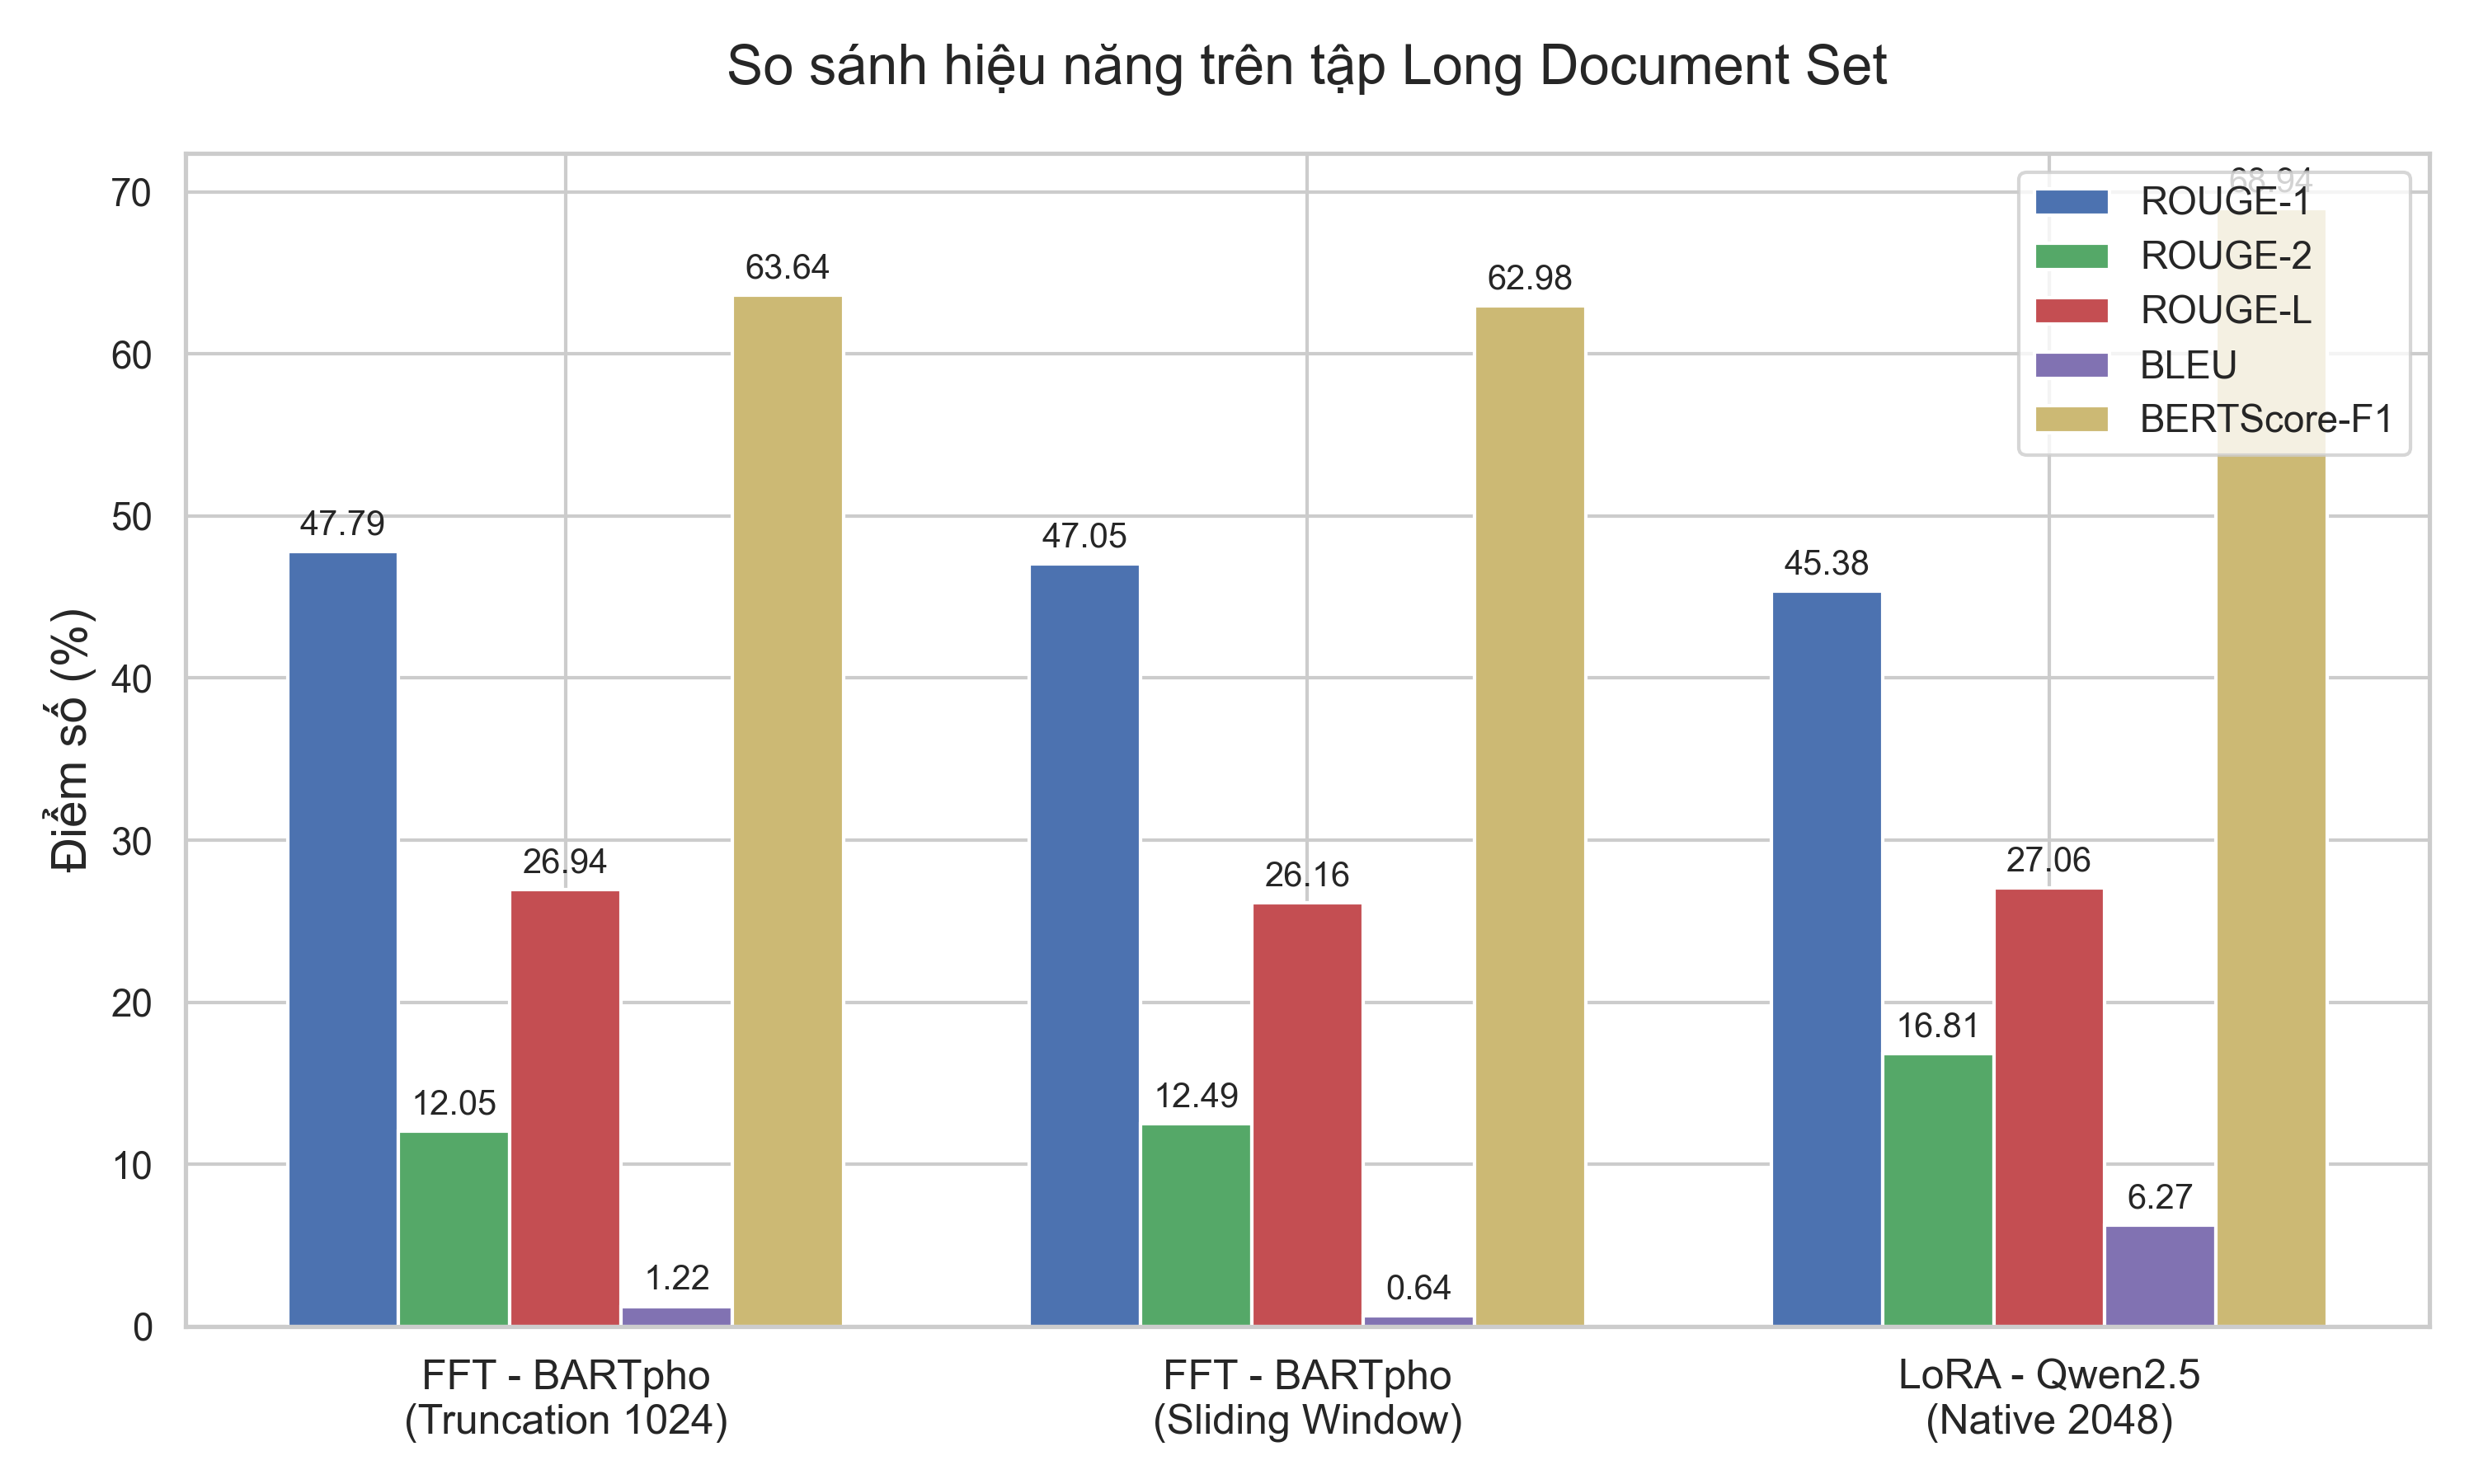
\includegraphics[width=\textwidth]{Images/long_context_metrics.png}
    \caption{So sánh hiệu năng trên tập văn bản dài. Phương pháp Map-Reduce đạt BLEU thấp nhất (0.64), trong khi Native Long-Context của Qwen2.5 duy trì BLEU ở mức 6.27.}
    \label{fig:long}
\end{figure}

\paragraph{Sự suy giảm hiệu năng của phương pháp Map-Reduce.}
Kết quả trong Bảng \ref{tab:long_eval} cho thấy phương pháp Sliding Window (Map-Reduce) đạt BLEU (0.64) và ROUGE-1 (47.05) thấp hơn so với phương pháp Normal Truncation (BLEU: 1.22, ROUGE-1: 47.79). Hiện tượng phản trực giác này -- kỹ thuật được thiết kế để xử lý văn bản dài lại cho kết quả kém hơn việc đơn giản cắt bỏ -- được giải thích qua hai nguyên nhân. Thứ nhất, do tác động của Lead Bias, phần đuôi bài báo thường chứa ít thông tin trọng tâm so với phần mở đầu; Normal Truncation vô tình tập trung vào phần giàu thông tin nhất. Thứ hai, quá trình tóm tắt phân cấp qua hai bước tạo ra hiện tượng mất mát thông tin tích lũy (Information Bottleneck): ở bước Map, mỗi đoạn cục bộ chỉ được tóm tắt với $\text{max\_length} = 64$ tokens -- một hạn chế nghiêm ngặt buộc mô hình phải loại bỏ nhiều thông tin ngữ cảnh. Khi các bản tóm tắt cục bộ được ghép nối ở bước Reduce, văn bản kết quả thiếu tính mạch lạc do mất liên kết ngữ cảnh chéo giữa các đoạn, dẫn đến BLEU giảm mạnh.

\paragraph{Ưu thế của Native Long-Context.}
Qwen2.5 duy trì BLEU ở mức 6.27, cao hơn gần 10 lần so với phương pháp Map-Reduce (0.64) và gấp 5 lần Normal Truncation (1.22). ROUGE-2 (16.81) cao hơn đáng kể so với cả hai cấu hình BARTpho (12.05 và 12.49), phản ánh khả năng bắt cụm từ liên tiếp (bigram) tốt hơn. BERTScore (68.94) cũng vượt trội (+5.30 so với BARTpho Normal Truncation), cho thấy độ tương đồng ngữ nghĩa cao hơn. Kết quả này phản ánh lợi thế của việc xử lý ngữ cảnh liền mạch: toàn bộ 2048 tokens được nạp vào mô hình trong một lần forward pass, cho phép cơ chế Self-Attention tạo kết nối trực tiếp giữa mọi cặp vị trí trong văn bản -- từ thông tin đầu bài đến kết luận cuối bài -- mà không bị phân mảnh. Tuy nhiên, cần thận trọng khi quy kết toàn bộ sự vượt trội này cho cơ chế Native Long-Context, bởi Qwen2.5 đồng thời được hưởng lợi từ quy mô dữ liệu tiền huấn luyện lớn hơn nhiều bậc (18T tokens so với 20GB) và bộ từ vựng BPE phong phú hơn ($\sim$152k so với $\sim$40k).

Mặt khác, ROUGE-1 của Qwen2.5 (45.38) thấp hơn BARTpho Normal Truncation (47.79, $\Delta = -2.41$). Xu hướng này nhất quán với quan sát trên General Set: Qwen2.5 có xu hướng sinh văn bản trừu tượng hơn, sử dụng paraphrase thay vì sao chép trực tiếp, dẫn đến trùng lặp unigram thấp hơn nhưng BLEU và BERTScore cao hơn nhờ cấu trúc câu mạch lạc và ý nghĩa ngữ cảnh được bảo toàn tốt hơn.

\subsection{Đánh giá Chất lượng Sinh bằng LLM-as-a-Judge}\label{sec:llm_judge}

Bên cạnh các độ đo tự động truyền thống, chúng tôi áp dụng phương pháp LLM-as-a-Judge sử dụng mô hình Gemini 3.5 Flash-Lite (được tối ưu hóa cho tốc độ và hiệu quả chi phí) để đánh giá đa chiều chất lượng văn bản sinh ra trên một tập mẫu ngẫu nhiên gồm 100 bài báo từ tập kiểm thử chung. Mỗi cặp (bài báo gốc, bản tóm tắt) được đưa vào prompt yêu cầu mô hình chấm điểm trên thang 1--5 cho 4 tiêu chí: Sự liên quan (Relevance -- bản tóm tắt có bao quát đúng các ý chính không?), Tính mạch lạc (Coherence -- cấu trúc logic giữa các câu), Tính nhất quán (Consistency -- không chứa thông tin bịa đặt so với bài gốc), và Độ trôi chảy (Fluency -- ngữ pháp, chính tả, hành văn tự nhiên). Mô hình được yêu cầu trả về kết quả dưới định dạng JSON chuẩn hóa, nhằm đảm bảo tính nhất quán trong phân tích. Bảng \ref{tab:llm_judge} và Hình \ref{fig:llm_judge} trình bày kết quả.

\begin{table}[H]
\centering
\caption{Kết quả đánh giá LLM-as-a-Judge trên thang điểm 1-5. Giá trị in đậm biểu thị kết quả tốt nhất trong các mô hình tiền huấn luyện.}
\label{tab:llm_judge}
\begin{tabular}{@{}lcccc@{}}
\toprule
\textbf{Phương pháp} & \textbf{Relevance} & \textbf{Coherence} & \textbf{Consistency} & \textbf{Fluency} \\
\midrule
FFT -- BARTpho & 2.75 & \textbf{3.51} & \textbf{4.05} & 2.76 \\
LoRA -- Qwen2.5 & 2.54 & 2.29 & 3.37 & 2.74 \\
LoRA -- Qwen2.5 + GTF & \textbf{2.80} & 2.72 & 3.57 & \textbf{3.31} \\
\midrule
Entity Guided + GTF (Custom) & 1.05 & 1.28 & 1.02 & 1.58 \\
\bottomrule
\end{tabular}
\end{table}

  \begin{figure}[H]
      \centering
      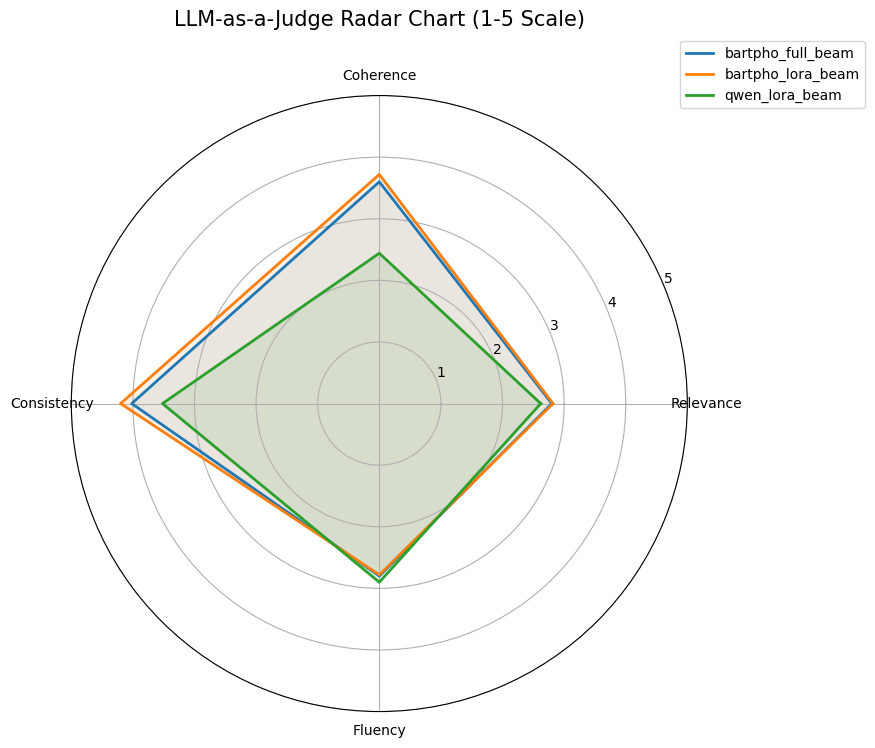
\includegraphics[width=0.7\textwidth]{Images/llm_judge.png}
      \caption{Biểu đồ so sánh điểm số LLM-as-a-Judge trên 4 tiêu chí.}
      \label{fig:llm_judge}
  \end{figure}

\paragraph{Sự lột xác của Causal LM nhờ thuật toán GTF.} 
Kết quả chấm điểm minh chứng rất rõ rệt cho hiện tượng kẹt lặp (Exposure Bias) của Causal LM và sức mạnh của thuật toán GTF-Penalty. Khi chưa có GTF, \textbf{LoRA -- Qwen2.5} có điểm Tính mạch lạc (Coherence) cực thấp (2.29) do hiện tượng sinh từ lặp lại luẩn quẩn, làm đứt gãy cấu trúc logic của văn bản. Tuy nhiên, sau khi áp dụng \textbf{GTF-Penalty}, mô hình đã có sự lột xác toàn diện: điểm Coherence tăng vọt lên 2.72, Độ trôi chảy (Fluency) vọt lên mức cao nhất bảng (3.31), và Sự liên quan (Relevance) cũng vượt lên dẫn đầu (2.80). Điều này khẳng định cơ chế phạt tần suất suy giảm cấu hình cục bộ không chỉ giải quyết triệt để lỗi lặp từ, mà còn "cởi trói" cho sức mạnh tiềm tàng của kiến trúc Causal LM, giúp nó sinh ra các câu văn tự nhiên và đi thẳng vào trọng tâm.

\paragraph{Vai trò của LLM-as-a-Judge trong đánh giá ngữ nghĩa.}
Kết quả đánh giá của mô hình \textbf{Entity Guided + GTF (Custom)} cho thấy sự bổ trợ cần thiết của phương pháp LLM-as-a-Judge đối với các thước đo tự động. Dù đạt ROUGE-1 50.00, mô hình này ghi nhận điểm đánh giá ngữ nghĩa rất thấp (Consistency = 1.02, Relevance = 1.05). Sự khác biệt này xảy ra do thước đo N-gram (như ROUGE) tập trung vào mức độ trùng lặp từ vựng mà không xem xét cấu trúc câu hay tính logic. 

Như đã phân tích ở Mục \ref{sec:general_eval}, Custom Transformer tập trung trích xuất các từ khóa đặc trưng (ví dụ: \textit{"Quân đội Nga"}, \textit{"Syria"}) để tăng N-gram. Tuy nhiên, vì thiếu nền tảng biểu diễn ngôn ngữ từ dữ liệu tiền huấn luyện lớn (như 20GB của BARTpho hay 18 nghìn tỷ token của Qwen2.5), mô hình gặp khó khăn trong việc xây dựng câu đúng ngữ pháp, dẫn đến hiện tượng câu kết thúc đột ngột hoặc sai lệch ngữ nghĩa so với văn bản gốc. Phương pháp LLM-as-a-Judge đã nhận diện chính xác hạn chế này bằng cách đánh giá dựa trên mức độ trôi chảy và tính nhất quán. Kết quả trên khẳng định rằng trong đánh giá tóm tắt văn bản, cần kết hợp cả thước đo từ vựng (ROUGE) và đánh giá ngữ nghĩa (LLM-as-a-Judge) để phản ánh đúng chất lượng tạo sinh thực tế thay vì chỉ dựa vào độ trùng lặp từ khóa rời rạc.

\subsection{Phân tích Lỗi (Error Analysis)}

Để làm rõ hơn các yếu điểm của mô hình, chúng tôi tiến hành phân tích lỗi chuyên sâu trên hai phương diện: sự ảnh hưởng của độ dài văn bản gốc và hiện tượng suy thoái sinh văn bản (text degeneration/hallucination).

\paragraph{Tác động của độ dài văn bản đầu vào.} 
Dữ liệu kiểm thử được phân loại thành ba nhóm theo độ dài: ngắn ($<300$ từ), trung bình ($300-600$ từ), và dài ($>600$ từ). Kết quả đo lường cho thấy hiệu năng của Qwen2.5 tỷ lệ nghịch với độ dài văn bản. Ở nhóm văn bản ngắn, ROUGE-1 của Qwen2.5 đạt 49.85 (thấp hơn BARTpho $\sim$1.2 điểm). Tuy nhiên, với nhóm văn bản $>600$ từ, chỉ số này giảm xuống 42.94, tạo khoảng cách 6.4 điểm so với mức 49.32 của BARTpho. Sự chênh lệch này cho thấy phiên bản Qwen2.5 Base gặp giới hạn trong việc phân bổ sự chú ý (attention allocation) đối với chuỗi ngữ cảnh dài khi chưa qua bước tinh chỉnh chỉ thị (Instruction Tuning) cho bài toán tóm tắt. Trong khi đó, kiến trúc Seq2Seq của BARTpho duy trì hiệu năng ổn định hơn (giảm từ 51.06 xuống 49.32).

\paragraph{Tỷ lệ lặp cấu trúc (Trigram Repetition Rate).}
Để định lượng hiện tượng suy thoái sinh văn bản (text degeneration), chúng tôi sử dụng Tỷ lệ lặp Trigram. Dữ liệu cho thấy BARTpho có tỷ lệ lặp thấp, đạt 0.55\% ở cấu hình FFT và 0.69\% ở cấu hình LoRA. Trái lại, mô hình Qwen2.5 gốc ghi nhận tỷ lệ lặp 10.32\%. Hiện tượng lặp cục bộ (local degeneration) này không chỉ làm giảm điểm LLM-as-a-Judge ở tiêu chí Mạch lạc và Nhất quán, mà còn hạn chế khả năng bao phủ từ vựng mới của văn bản đầu ra, dẫn đến chỉ số ROUGE-1 thấp. Việc tích hợp thuật toán GTF-Penalty (phân tích tại Mục 5.2) là phương pháp giải quyết hiện tượng này, giúp kiểm soát tỷ lệ lặp và cải thiện chất lượng sinh văn bản của kiến trúc Causal LLM.

%======================================================================
\section{Phạm vi và Hạn chế}
\label{sec:limitations}
%======================================================================

Nghiên cứu này được thực hiện với một số giới hạn về phạm vi và tài nguyên cần được thừa nhận rõ ràng. 

\paragraph{Phạm vi dữ liệu và Phương pháp đánh giá.} 
Tập dữ liệu huấn luyện được giới hạn ở 10,000 mẫu trong miền tin tức (VietNews), do đó khả năng tổng quát hóa (generalizability) của các mô hình sang các miền chuyên sâu như y tế hay pháp luật chưa được kiểm chứng. Về mặt đánh giá, mặc dù chúng tôi đã tích hợp LLM-as-a-Judge, sự tham gia của con người (Human Evaluation) vẫn là tiêu chuẩn vàng chưa được thực hiện để đánh giá trọn vẹn các sắc thái văn phong báo chí. Bên cạnh đó, việc sử dụng mô hình đa ngôn ngữ \texttt{bert-base-multilingual-cased} cho đo lường BERTScore thay vì một mô hình đơn ngữ tối ưu riêng cho tiếng Việt (như PhoBERT \cite{phobert}) cũng là một điểm có thể được nâng cấp trong tương lai.

\paragraph{Giới hạn phần cứng và Thiết lập thực nghiệm.} 
Dưới ràng buộc của GPU T4 (16GB VRAM), thiết lập so sánh giữa BARTpho và Qwen2.5 chưa hoàn toàn đối xứng. Trong khi BARTpho có thể thực hiện Full Fine-Tuning (FFT) nhờ kiến trúc Encoder-Decoder tối ưu bộ nhớ, Qwen2.5 (Decoder-only) chỉ có thể huấn luyện với LoRA và effective batch size nhỏ hơn do yêu cầu lưu trữ KV-Cache rất lớn cho chuỗi ngữ cảnh dài (2048 tokens). Ngoài ra, quyết định sử dụng phiên bản BARTpho syllable-level nhằm đơn giản hóa pipeline tiền xử lý (không phụ thuộc external word segmenter) đã đánh đổi bằng việc thu hẹp cửa sổ ngữ cảnh hiệu dụng. Cuối cùng, dù phương pháp Paired Bootstrap Resampling đã được áp dụng để xác nhận ý nghĩa thống kê cho các phát hiện chính, một số chênh lệch vi mô (như $\Delta$ ROUGE-1 = 0.07 giữa FFT và LoRA) vẫn nằm trong ranh giới của dao động ngẫu nhiên và cần được độc giả diễn giải thận trọng.

\paragraph{Khảo sát Kiến trúc Trạng thái Chọn lọc (Selective State Spaces).}
Mặc dù nghiên cứu này đã thiết kế và đánh giá kiến trúc Transformer tùy chỉnh, chúng tôi cũng ghi nhận sự trỗi dậy của các mô hình Mamba \cite{mamba_custom}. Phân tích thực nghiệm của chúng tôi chỉ ra rằng trong bài toán tóm tắt tiếng Việt với độ dài trung bình, cơ chế nén trạng thái cố định của Mamba (quét tuyến tính) có thể trở thành nút cổ chai thông tin đối với các tín hiệu thưa (như danh từ riêng, số liệu). Trái lại, đồ thị liên kết toàn cục (Global Attention) của Transformer bảo toàn tín hiệu thực thể tốt hơn. Việc đánh giá chuyên sâu mô hình Mamba trên ngữ cảnh siêu dài là một giới hạn mở nằm ngoài phạm vi hiện tại.

%======================================================================
\section{Kết luận và Hướng phát triển}
\label{sec:conclusion}
%======================================================================

Nghiên cứu này đã thực hiện đánh giá toàn diện bài toán tóm tắt văn bản tiếng Việt trên tập dữ liệu VietNews, so sánh ba thế hệ phương pháp từ trích xuất truyền thống đến mô hình ngôn ngữ lớn. Bảng \ref{tab:rq_summary} tổng kết các phát hiện chính theo ba câu hỏi nghiên cứu.

\begin{table}[H]
\centering
\caption{Tổng kết các phát hiện theo câu hỏi nghiên cứu.}
\label{tab:rq_summary}
\begin{tabular}{@{}p{1.5cm}p{4cm}p{8cm}@{}}
\toprule
\textbf{RQ} & \textbf{Câu hỏi} & \textbf{Phát hiện chính} \\
\midrule
RQ1 & Cải tiến cấu trúc lõi và GTF-Penalty & Việc thay thế cấu trúc (RoPE, RMSNorm, SwiGLU) và phạt lặp từ (GTF-Penalty) giúp tăng vọt ROUGE-1 từ 34.37 lên 50.00 ở mô hình huấn luyện từ đầu \\
RQ2 & Seq2Seq vs. Causal LLM & Qwen2.5 kết hợp GTF-Penalty đạt đỉnh SOTA trên mọi chỉ số sinh (ROUGE-1: 51.28, BLEU: 10.29), vượt qua hoàn toàn BARTpho (ROUGE-1: 50.24, BLEU: 2.25) \\
RQ3 & LoRA vs. Full Fine-Tuning & LoRA tiệm cận FFT ($\Delta$ ROUGE-1 = 0.07, tương đương 0.14\%) với $<$5\% tham số \\
RQ4 & Sliding Window vs. Native Long-Context & Native Long-Context vượt trội (BLEU 6.27 vs 0.64), Map-Reduce gây Information Bottleneck \\
\bottomrule
\end{tabular}
\end{table}

Đối với RQ1, các cải tiến từ cấp độ phép toán lõi đến kiến trúc và thuật toán giải mã mang lại hiệu năng ấn tượng cho mô hình huấn luyện từ đầu. Đặc biệt, GTF-Penalty là một giải pháp can thiệp suy diễn hiệu quả, chi phí thấp nhằm khắc phục exposure bias.

Đối với RQ2, Qwen2.5 thể hiện sức mạnh vượt trội khi kết hợp tinh chỉnh LoRA và GTF-Penalty. Mặc dù BARTpho vốn là mô hình được thiết kế chuyên biệt cho học Seq2Seq và bao phủ từ vựng tốt (ROUGE-1: 50.24), Qwen2.5+GTF vẫn thiết lập mức đỉnh SOTA trên mọi chỉ số đánh giá: ROUGE-1 51.28, ROUGE-2 23.05, BLEU 10.29 (vượt xa 2.25 của BARTpho) và BERTScore tiệm cận phương pháp trích xuất Lead-3. Sự vượt trội này khẳng định xu hướng LLM kiến trúc Causal Decoder kích thước trung bình (0.5B), nếu được giải mã đúng cách để chống lặp từ, có thể thay thế hoàn toàn các kiến trúc Encoder-Decoder truyền thống trong bài toán tóm tắt tiếng Việt. Tuy nhiên, cũng cần lưu ý rằng sự khác biệt này chịu ảnh hưởng đồng thời từ quy mô dữ liệu tiền huấn luyện (18T tokens so với 20GB), bộ tokenizer (BPE so với syllable), và hiệu năng có thể không hoàn toàn do kiến trúc.

Đối với RQ3, LoRA đạt hiệu năng tiệm cận Full Fine-Tuning (chênh lệch ROUGE-1 chỉ 0.07 điểm, tương đương 0.14\%) trong khi giảm trên 95\% lượng tham số cần cập nhật, khẳng định tính khả thi của kỹ thuật PEFT trong môi trường tài nguyên hạn chế. Kết quả này nhất quán với kết luận lý thuyết của Hu et al. \cite{lora} rằng không gian cập nhật hiệu quả có chiều thấp hơn nhiều so với toàn bộ không gian tham số.

Đối với RQ4, Qwen2.5 với cơ chế Native Long-Context cho thấy ưu thế rõ ràng trên văn bản dài, đạt BLEU 6.27 (gấp gần 10 lần so với phương pháp Map-Reduce của BARTpho ở mức 0.64), mặc dù sự vượt trội này cũng chịu ảnh hưởng từ các yếu tố ngoài cơ chế ngữ cảnh (quy mô pre-training, tokenizer). Đáng chú ý, Map-Reduce không cải thiện mà còn làm suy giảm chất lượng so với Normal Truncation do hiện tượng Information Bottleneck tích lũy qua hai bước tóm tắt, kết hợp với Lead Bias khiến phần đuôi bài báo đóng góp ít thông tin hữu ích.

Hướng phát triển tiếp theo bao gồm: (i) tiến hành đánh giá bởi con người (Human Evaluation) phối hợp cùng chuyên gia ngôn ngữ để kiểm chứng kết quả từ LLM-as-a-Judge; (ii) mở rộng thử nghiệm sang các phiên bản Qwen2.5-Instruct hoặc các mô hình lớn hơn (1.5B, 3B) để khắc phục điểm yếu về Coherence và Relevance của mô hình Base; (iii) thử nghiệm trên dữ liệu đa miền (y tế, pháp luật) để kiểm chứng khả năng tổng quát hóa; và (iv) áp dụng kỹ thuật QLoRA \cite{qlora} để tinh chỉnh trên cấu hình phần cứng hạn chế.

%======================================================================
\section*{Đóng góp của các tác giả}
\addcontentsline{toc}{section}{Đóng góp của các tác giả}
%======================================================================

\textbf{Nguyễn Đình Đạt} đóng vai trò trưởng nhóm nghiên cứu, chịu trách nhiệm lên ý tưởng, thiết kế phương pháp luận tổng thể và quản lý dự án. Tác giả đã thực hiện việc chuẩn bị, tiền xử lý dữ liệu, đồng thời xây dựng hệ thống pipeline đánh giá. Về mặt thực nghiệm, tác giả trực tiếp huấn luyện mô hình BARTpho, triển khai tinh chỉnh họ mô hình Qwen, và phát triển kỹ thuật GTF-Penalty. Tác giả cũng phụ trách phân tích kết quả định lượng, xây dựng ứng dụng Web Demo, và chắp bút bản thảo chính của bài báo, ngoại trừ phần kiến trúc mô hình.

\textbf{Lương Thành Vinh} chịu trách nhiệm chính về mảng kiến trúc mô hình học sâu. Tác giả đã trực tiếp tham gia xây dựng, tối ưu hóa Custom Transformer, và đề xuất các phương pháp cải tiến chuyên sâu về cơ chế Attention. Về mặt học thuật, tác giả đảm nhận việc soạn thảo và hoàn thiện toàn bộ phần Phương pháp luận liên quan đến kiến trúc Transformer trong bài báo.

\textbf{Bùi Đức Nhật} đóng vai trò then chốt trong việc khảo sát tài liệu và định hướng các dòng mô hình ngôn ngữ lớn ứng dụng cho đề tài. Tác giả phụ trách toàn bộ quy trình kiểm thử, thu thập log và xác thực kết quả thực nghiệm chuyên sâu cho nhánh kiến trúc Transformer. Bên cạnh đó, tác giả còn trực tiếp tham gia hỗ trợ triển khai và vận hành hệ thống Web Demo tương tác. Về công tác tổng kết, tác giả chịu trách nhiệm rà soát, tinh chỉnh chất lượng bản thảo và thiết kế hệ thống tài liệu thuyết trình trực quan phục vụ báo cáo hội đồng.

\newpage
% --- TÀI LIỆU THAM KHẢO ---
\renewcommand{\refname}{Tài liệu tham khảo}
\begin{thebibliography}{25}

\bibitem{vietnews}
Nguyen, T.-C., Nguyen, H.-D., \& Nguyen, V.-H. (2019).
\textit{VNDS: A Vietnamese Dataset for Summarization}.
Available at: \texttt{https://huggingface.co/datasets/nam194/vietnews}.

\bibitem{bartpho}
Tran, N. Q., et al. (2022).
\textit{BARTpho: Pre-trained Sequence-to-Sequence Models for Vietnamese}.
Proceedings of INTERSPEECH 2022.

\bibitem{qwen25}
Qwen Team (2024).
\textit{Qwen2.5 Technical Report}.
arXiv preprint arXiv:2412.15115.

\bibitem{lora}
Hu, E. J., et al. (2022).
\textit{LoRA: Low-Rank Adaptation of Large Language Models}.
Proceedings of ICLR 2022.

\bibitem{vaswani2017}
Vaswani, A., et al. (2017).
\textit{Attention Is All You Need}.
Advances in Neural Information Processing Systems (NeurIPS).

\bibitem{bart_original}
Lewis, M., et al. (2020).
\textit{BART: Denoising Sequence-to-Sequence Pre-training for Natural Language Generation, Translation, and Comprehension}.
Proceedings of ACL 2020.

\bibitem{lead_bias}
Kryściński, W., et al. (2019).
\textit{Neural Text Summarization: A Critical Evaluation}.
Proceedings of EMNLP 2019.

\bibitem{bertscore}
Zhang, T., et al. (2020).
\textit{BERTScore: Evaluating Text Generation with BERT}.
Proceedings of ICLR 2020.

\bibitem{rope}
Su, J., et al. (2024).
\textit{RoFormer: Enhanced Transformer with Rotary Position Embedding}.
Neurocomputing, 568, 127063.

\bibitem{rouge_original}
Lin, C.-Y. (2004).
\textit{ROUGE: A Package for Automatic Evaluation of Summaries}.
Proceedings of the ACL Workshop on Text Summarization.

\bibitem{bleu_original}
Papineni, K., et al. (2002).
\textit{BLEU: a Method for Automatic Evaluation of Machine Translation}.
Proceedings of ACL 2002.

\bibitem{textrank}
Mihalcea, R. \& Tarau, P. (2004).
\textit{TextRank: Bringing Order into Texts}.
Proceedings of EMNLP 2004.

\bibitem{map_reduce_summarization}
Ravaut, M., et al. (2023).
\textit{On Context Utilization in Summarization with Large Language Models}.
arXiv preprint arXiv:2310.10570.

\bibitem{phobert}
Nguyen, D. Q. \& Nguyen, A. T. (2020).
\textit{PhoBERT: Pre-trained Language Models for Vietnamese}.
Findings of EMNLP 2020.

\bibitem{mbart}
Liu, Y., et al. (2020).
\textit{Multilingual Denoising Pre-training for Neural Machine Translation}.
Transactions of the ACL, 8, 726--742.

\bibitem{mt5}
Xue, L., et al. (2021).
\textit{mT5: A Massively Multilingual Pre-trained Text-to-Text Transformer}.
Proceedings of NAACL 2021.

\bibitem{qlora}
Dettmers, T., et al. (2023).
\textit{QLoRA: Efficient Finetuning of Quantized Large Language Models}.
Proceedings of NeurIPS 2023.

\bibitem{prefix_tuning}
Li, X. L. \& Liang, P. (2021).
\textit{Prefix-Tuning: Optimizing Continuous Prompts for Generation}.
Proceedings of ACL 2021.

\bibitem{adapter}
Houlsby, N., et al. (2019).
\textit{Parameter-Efficient Transfer Learning for NLP}.
Proceedings of ICML 2019.

\bibitem{pagerank}
Brin, S. \& Page, L. (1998).
\textit{The Anatomy of a Large-Scale Hypertextual Web Search Engine}.
Computer Networks, 30(1-7), 107--117.

\bibitem{lexrank}
Erkan, G. \& Radev, D. R. (2004).
\textit{LexRank: Graph-based Lexical Centrality as Salience in Text Summarization}.
Journal of Artificial Intelligence Research, 22, 457--479.

\bibitem{gpt3}
Brown, T., et al. (2020).
\textit{Language Models are Few-Shot Learners}.
Advances in Neural Information Processing Systems (NeurIPS).

\bibitem{llama}
Touvron, H., et al. (2023).
\textit{LLaMA: Open and Efficient Foundation Language Models}.
arXiv preprint arXiv:2302.13971.

\bibitem{gqa}
Ainslie, J., et al. (2023).
\textit{GQA: Training Generalized Multi-Query Transformer Models from Multi-Head Checkpoints}.
Proceedings of EMNLP 2023.

\bibitem{vncorenlp}
Vu, T., et al. (2018).
\textit{VnCoreNLP: A Vietnamese Natural Language Processing Toolkit}.
Proceedings of NAACL 2018 -- Demonstrations.

\bibitem{rmsnorm_custom}
Zhang, B., \& Sennrich, R. (2019).
\textit{Root Mean Square Layer Normalization}.
Advances in Neural Information Processing Systems (NeurIPS).

\bibitem{swiglu_custom}
Shazeer, N. (2020).
\textit{GLU Variants Improve Transformer}.
arXiv preprint arXiv:2002.05202.

\bibitem{weight_tying_custom}
Press, O., \& Wolf, L. (2017).
\textit{Using the Output Embedding to Improve Language Models}.
Proceedings of EACL 2017.

\bibitem{label_smoothing_custom}
Szegedy, C., et al. (2016).
\textit{Rethinking the Inception Architecture for Computer Vision}.
Proceedings of CVPR 2016.

\bibitem{mamba_custom}
Gu, A., \& Dao, T. (2023).
\textit{Mamba: Linear-Time Sequence Modeling with Selective State Spaces}.
arXiv preprint arXiv:2312.00752.

\end{thebibliography}

\end{document}
